To improve the exclusion limit on the \brThb, the $\mjj$ from different 
event categories have been used for limit computation.
\section{Inclusive event category without charm tagging}
\label{ss:mjj_Inc}
The $\mjj$ distribution without further categorizing events based on charm 
tagging was used at 8 \TeV~\cite{Khachatryan:2015uua} for limit computation due 
to the unavailability of dedicated charm taggers. For sake of comparison, at 
13 \TeV also the exclusion limit is computed using $\mjj$ after kinematic fit
selection, without the charm tagging. The event yields are shown in Table
\ref{tab:eventYieldInc}. Corresponding $\mjj$ distributions are shown in 
Figures~\ref{subfig:mjj_kfit_muKinFit},~\ref{subfig:mjj_kfit_eleKinFit}, 
~\ref{subfig:mjj_sig_kfit_mu},~\ref{subfig:mjj_sig_kfit_ele}. The exclusion 
limit for inclusive event category is computed in Section~\ref{ss:limit_Inc}. 
\begin{table}
\caption{Event yield for inclusive category after kinematic fit selection. The statistical 
uncertainty in the total background corresponds to the quadratically added uncertainties from 
individual backgrounds. However, a systematic uncertainty correlated among each background is 
linearly added for the total background. And each uncorrelated systematic uncertainty
for the total background is quadratically added.}
\label{tab:eventYieldInc}
\begin{center}
\begin{tabular}{cccc}
\hline 
\hline 
\bf{Process}& $N_{\rm{events}} \pm \rm{stat} \pm \rm{sys}$ & $N_{\rm{events}} \pm \rm{stat} \pm \rm{sys}$\\ 
 & \mujets &  \ejets\\
\hline 
\hline 
$\mHp=80$ \GeV & 15578 $\pm$ 110 $\pm$ 1101 & 11736 $\pm$ 94 $\pm$ 844\\
$\mHp=90$ \GeV & 15721 $\pm$ 109 $\pm$ 1202 & 12076 $\pm$ 95 $\pm$ 899\\
$\mHp=100$ \GeV & 16321 $\pm$ 111 $\pm$ 1191 & 12206 $\pm$ 95 $\pm$ 826\\
$\mHp=120$ \GeV & 15719 $\pm$ 109 $\pm$ 1108 & 11805 $\pm$ 93 $\pm$ 830\\
$\mHp=140$ \GeV & 12461 $\pm$ 97 $\pm$ 996 & 9494 $\pm$ 84 $\pm$ 738\\
$\mHp=150$ \GeV & 8909 $\pm$ 82 $\pm$ 776 & 6902 $\pm$ 72 $\pm$ 630\\
$\mHp=155$ \GeV & 7014 $\pm$ 74 $\pm$ 713 & 5398 $\pm$ 64 $\pm$ 587\\
$\mHp=160$ \GeV & 5383 $\pm$ 64 $\pm$ 567 & 4184 $\pm$ 56 $\pm$ 451\\
\hline 
SM \ttjets & 191135 $\pm$ 268 $\pm$ 14066 & 141807 $\pm$ 228 $\pm$ 10492\\
Single \PQt & 5312 $\pm$ 40 $\pm$ 506 & 3989 $\pm$ 35 $\pm$ 405\\
QCD multijet & 4631 $\pm$ 240 & 3780 $\pm$ 179\\
\wjets & 2795 $\pm$ 123 $\pm$ 575 & 2032 $\pm$ 71 $\pm$ 289\\
\dyjets & 389 $\pm$ 15 $\pm$ 76 & 433 $\pm$ 15 $\pm$ 76\\
VV & 147 $\pm$ 20 $\pm$ 33 & 70 $\pm$ 13 $\pm$ 14\\
\hline 
All background & 204409 $\pm$ 383 $\pm$ 15153 & 152111 $\pm$ 301 $\pm$   11241\\
\hline 
Data & 203207 $\pm$ 451 & 148499 $\pm$ 385 \\
\hline 
\end{tabular}
\end{center}
\end{table}
    
\section{Inclusive event category with loose charm tagging}
\label{ss:mjj_cTagL}
The charm taggers as discussed in Section~\ref{s:cTag} are used to tag a jet 
as \PQc jet. After kinematic fit selection, one of the jets forming $\mjj$ is 
required to pass the \PQc tagging requirement. The event yields for loose charm 
working points after applying \PQc tag event weights are shown in Table~\ref{tab:eventYieldCTagInc}. 
The $\mjj$ distributions with inclusive loose charm tagging are 
shown in Figure~\ref{fig:mjj_cTagL}. Exclusion limits using $\mjj$ after 
applying loose charm tagging is computed in Section~\ref{ss:limit_cTagL}.
\begin{figure}
\centering  
\subfigure[\label{subfig:mjj_kfit_CTagIncL_muKinFit}]
{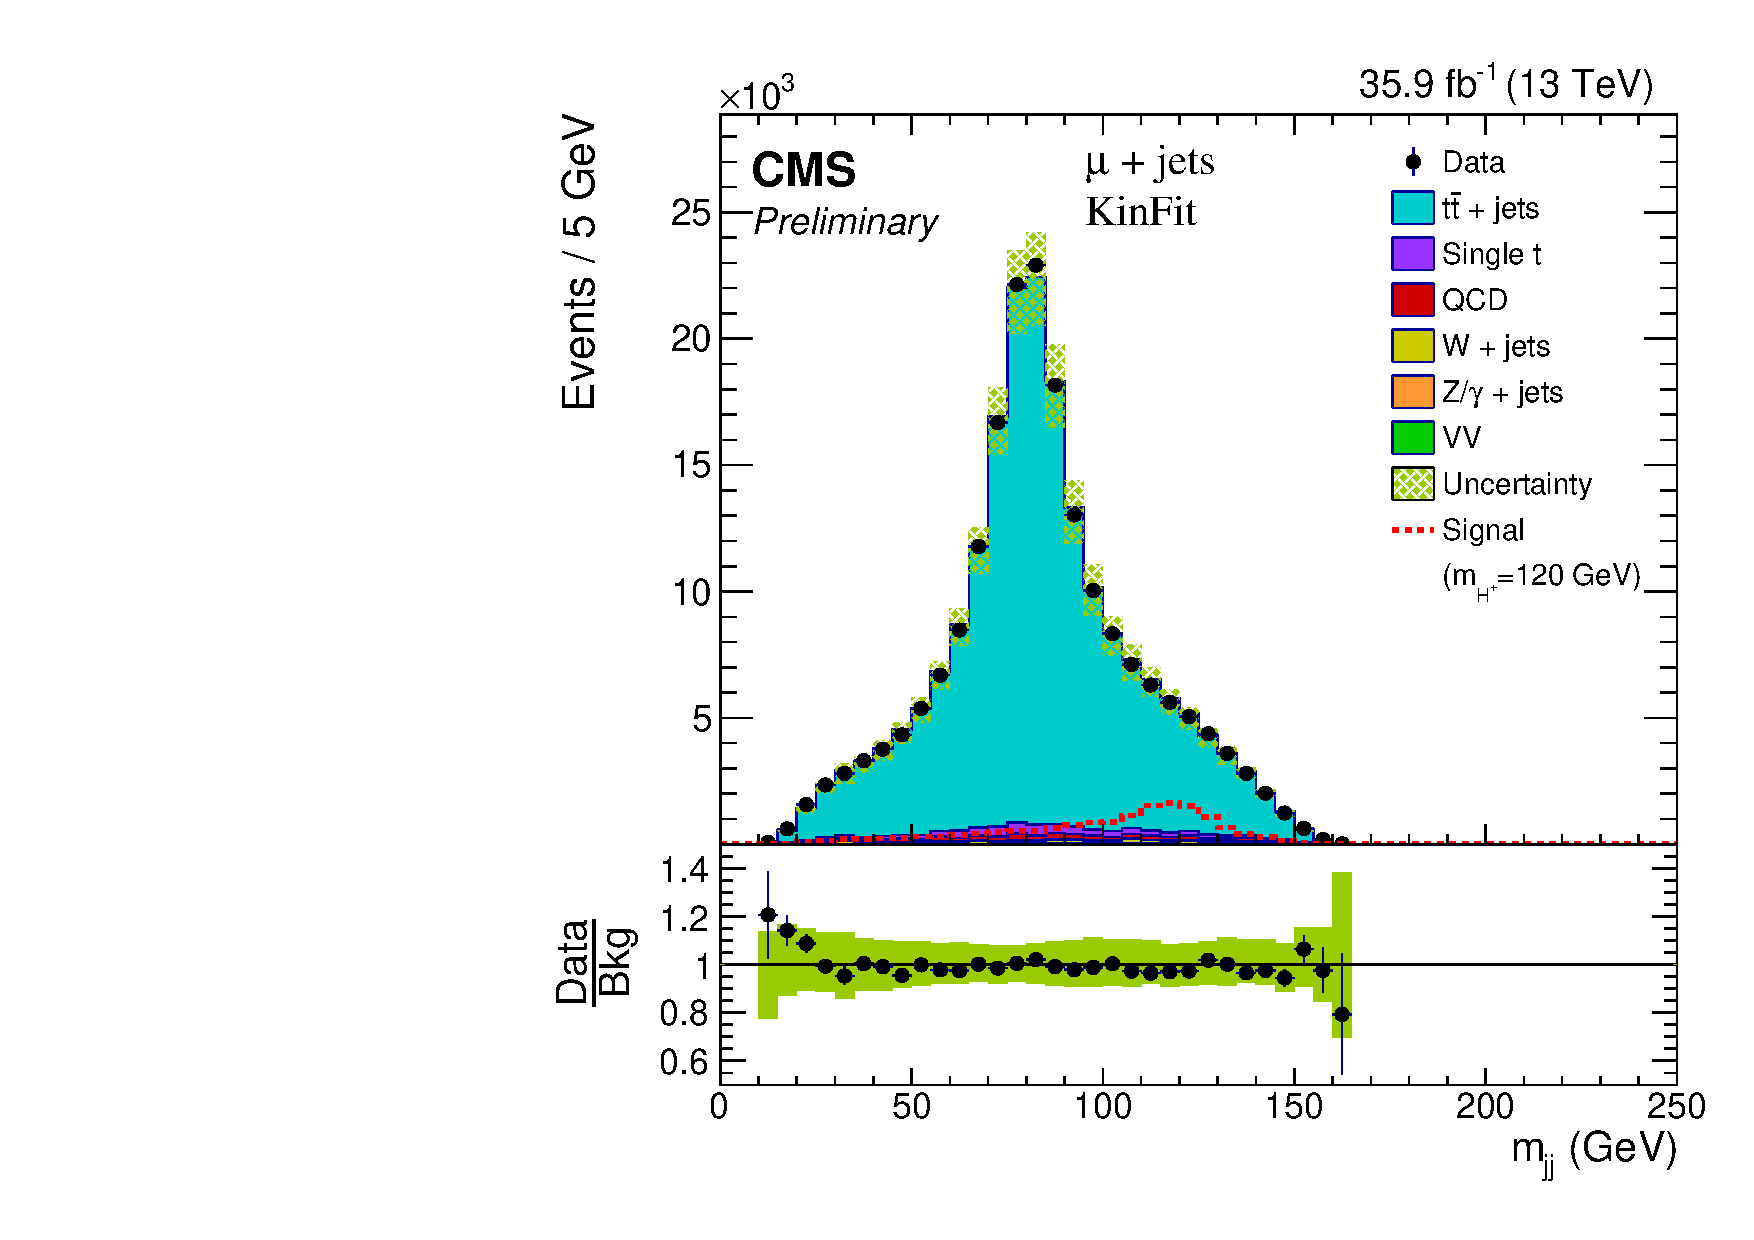
\includegraphics[width=0.49\linewidth]{Image/Muon/KinFit/mjj_kfit_CTagIncL_muKinFit.pdf}}
\subfigure[\label{subfig:mjj_kfit_CTagIncL_eleKinFit}]
{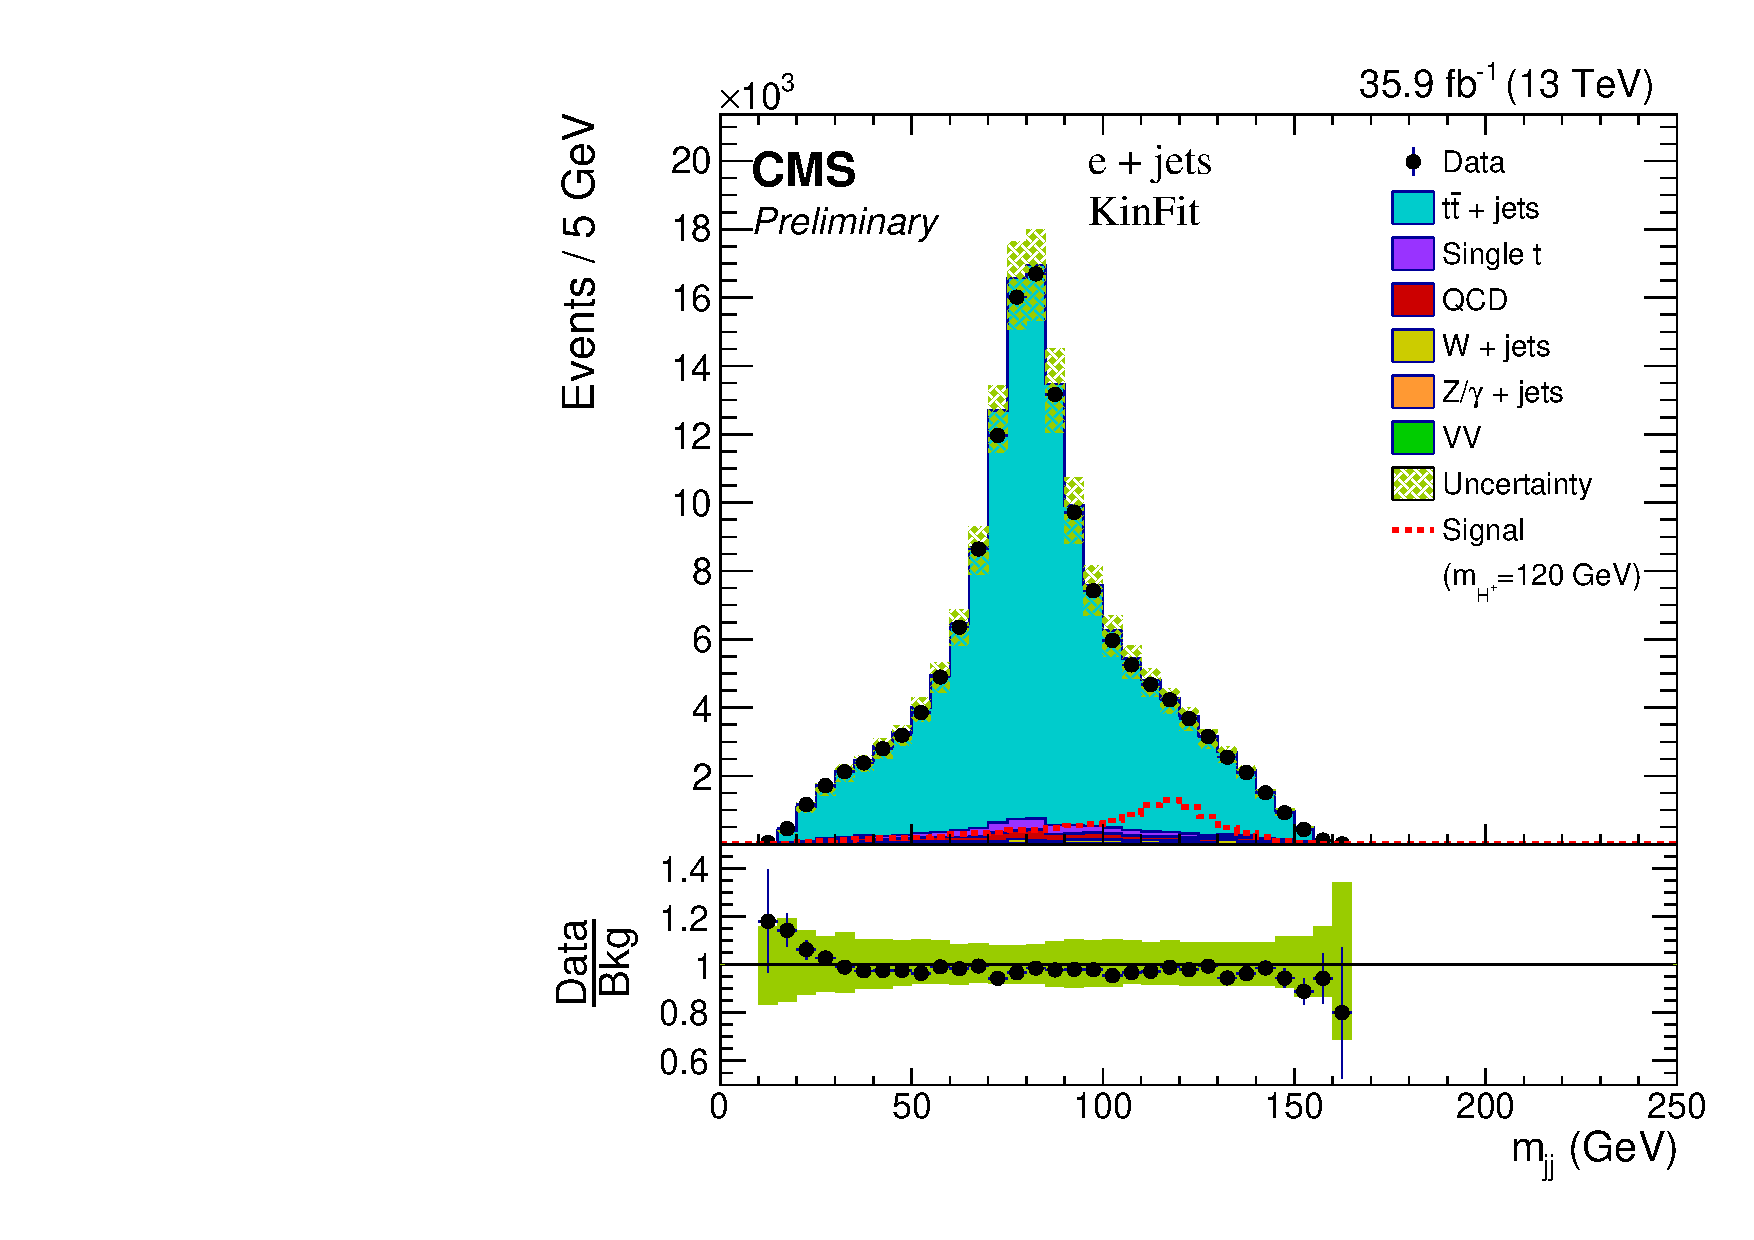
\includegraphics[width=0.49\linewidth]{Image/Electron/KinFit/mjj_kfit_CTagIncL_eleKinFit.pdf}}
\caption{Distribution of $\mjj$ for inclusive loose charm tagging as
described in Section~\ref{ss:mjj_cTagL} for \mujets and \ejets channel.}
\label{fig:mjj_cTagL}
\end{figure}

\begin{table}
\caption{Event yield for inclusive loose charm category after kinematic fit selection. 
The statistical uncertainty in the total background corresponds to the quadratically added 
uncertainties from individual backgrounds. However, a systematic uncertainty correlated 
among each background is linearly added for the total background. And each uncorrelated 
systematic uncertainty for the total background is quadratically added.}
\label{tab:eventYieldCTagInc}
\begin{center}
\begin{tabular}{cccc}
\hline 
\hline 
\bf{Process}& $N_{\rm{events}} \pm \rm{stat} \pm \rm{sys}$ & $N_{\rm{events}} \pm \rm{stat} \pm \rm{sys}$\\
 & \mujets &  \ejets\\
\hline 
\hline 
$\mHp=80$ \GeV & 15614 $\pm$ 111 $\pm$ 1405 & 11757 $\pm$ 95 $\pm$ 1054\\
$\mHp=90$ \GeV & 15733 $\pm$ 110 $\pm$ 1484 & 12076 $\pm$ 96 $\pm$ 1115\\
$\mHp=100$ \GeV & 16372 $\pm$ 112 $\pm$ 1488 & 12231 $\pm$ 96 $\pm$ 1081\\
$\mHp=120$ \GeV & 15785 $\pm$ 110 $\pm$ 1447 & 11835 $\pm$ 94 $\pm$ 1084\\
$\mHp=140$ \GeV & 12521 $\pm$ 98 $\pm$ 1281 & 9546 $\pm$ 85 $\pm$ 940\\
$\mHp=150$ \GeV & 8956 $\pm$ 83 $\pm$ 978 & 6937 $\pm$ 72 $\pm$ 781\\
$\mHp=155$ \GeV & 7057 $\pm$ 75 $\pm$ 907 & 5435 $\pm$ 65 $\pm$ 698\\
$\mHp=160$ \GeV & 5408 $\pm$ 65 $\pm$ 686 & 4205 $\pm$ 57 $\pm$ 539\\
\hline 
SM \ttjets & 190227 $\pm$ 269 $\pm$ 17385 & 141111 $\pm$ 229 $\pm$ 12842\\
Single \PQt & 5272 $\pm$ 40 $\pm$ 589 & 3954 $\pm$ 35 $\pm$ 464\\
QCD multijet & 4185 $\pm$ 226 & 3426 $\pm$ 172\\
\wjets & 2761 $\pm$ 121 $\pm$ 631 & 1991 $\pm$ 70 $\pm$ 330\\
\dyjets & 378 $\pm$ 15 $\pm$ 82 & 418 $\pm$ 15 $\pm$ 80\\
VV & 147 $\pm$ 20 $\pm$ 35 & 70 $\pm$ 13 $\pm$ 15\\
\hline 
All background & 202970 $\pm$ 375 $\pm$ 18612 & 150970 $\pm$ 297 $\pm$   13700\\
\hline 
Data & 201360 $\pm$ 449 & 147210 $\pm$ 384 \\
\hline 
\end{tabular}
\end{center}
\end{table}

\section{Exclusive event categories based on charm tagging}
\label{ss:mjj_cTagEx}
The signal significance is different in different charm working points as can 
be seen from Figure~\ref{fig:ratioSB_1} and \ref{fig:ratioSB_2}. This property is 
exploited in improving the exclusion limits. Events are exclusively divided in to 
the loose, medium, and tight categories as shown in Figure~\ref{fig:cTagCat}, based 
on whether one of the jets forming $\mjj$ pass loose but not medium, medium but not tight, 
and tight working points of the \PQc tagging requirements, respectively. The QCD multijet
events are estimated in each category following the procedure given in Chapter~\ref{s:secQCD}. 
The resulting $\mjj$ from various categories are combined to compute the limit. 
\begin{figure}
\centering  
\subfigure[]{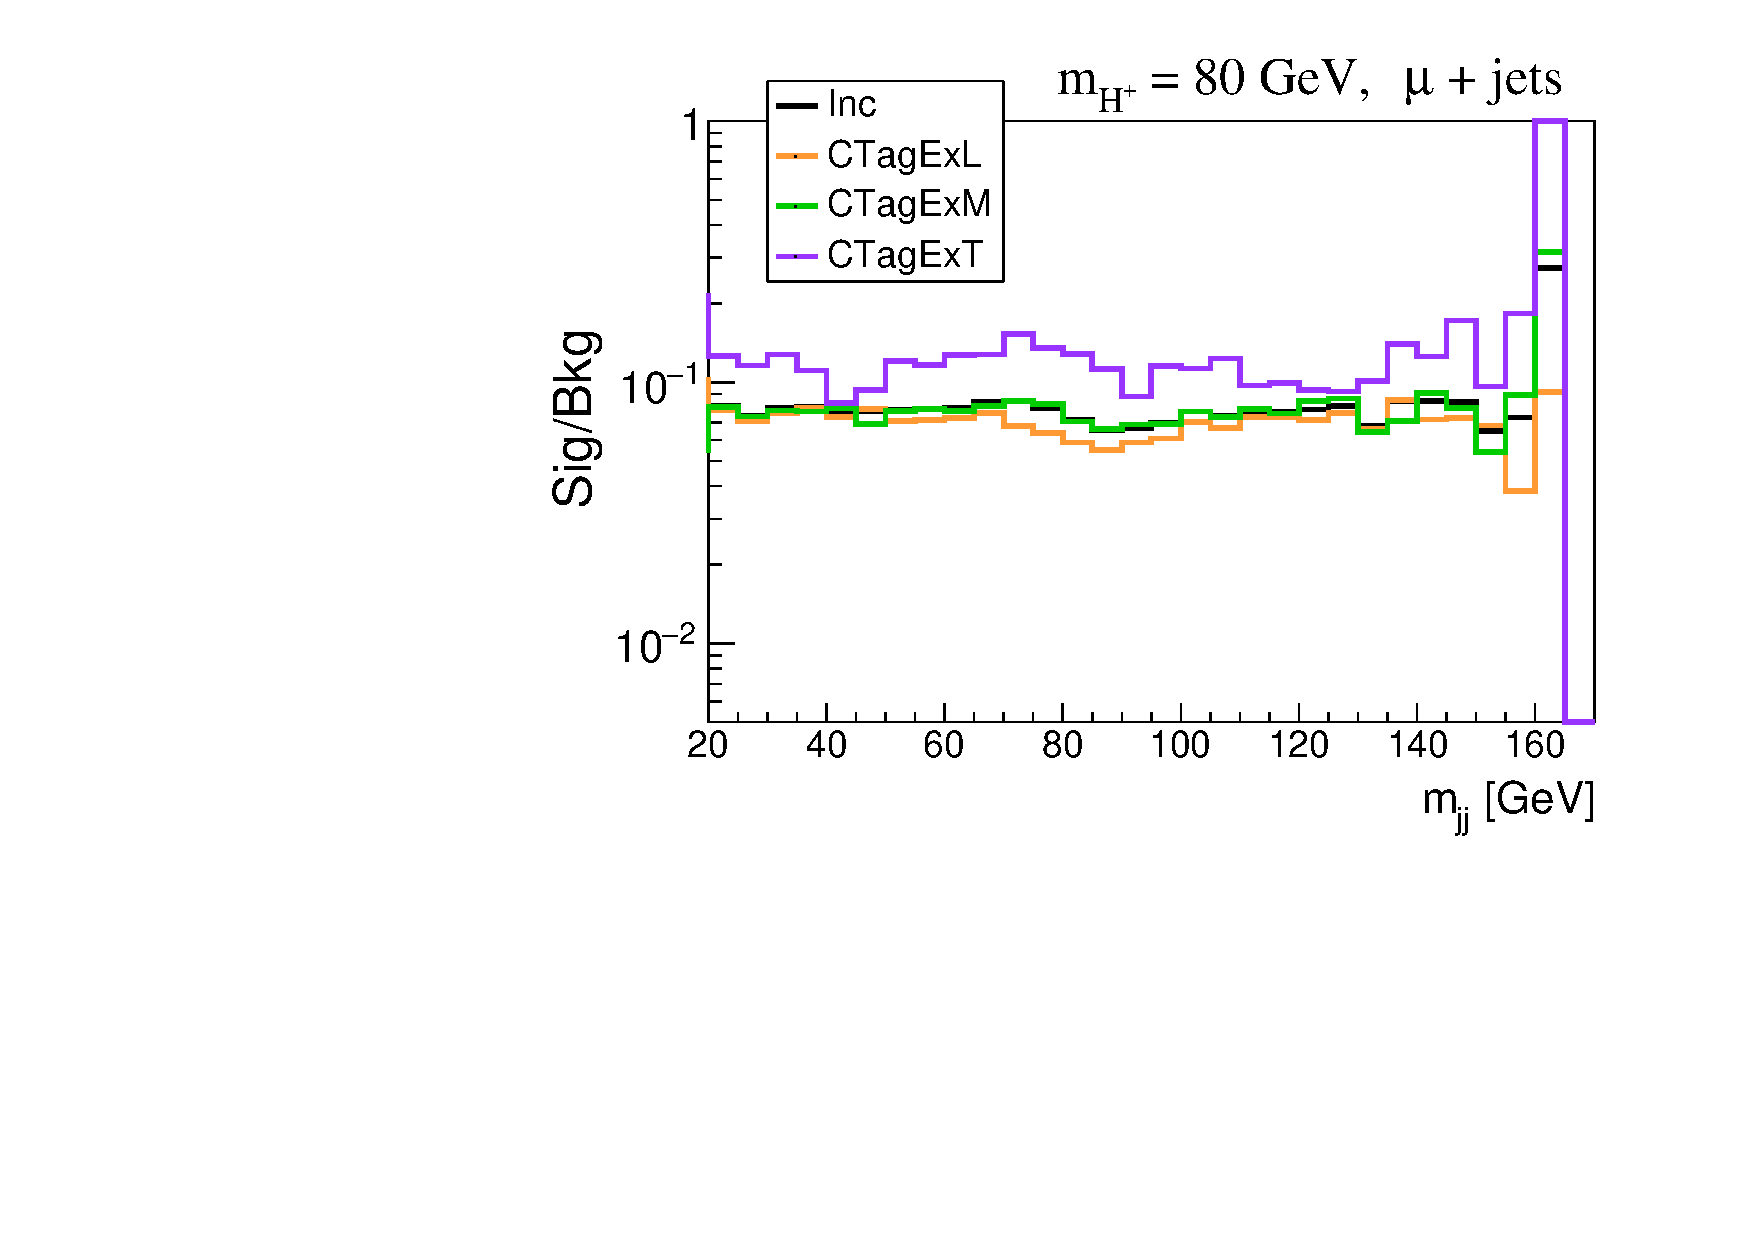
\includegraphics[width=0.40\linewidth]{Image/Muon/CTag/WH80_mu_ratioSB.pdf}}
\subfigure[]{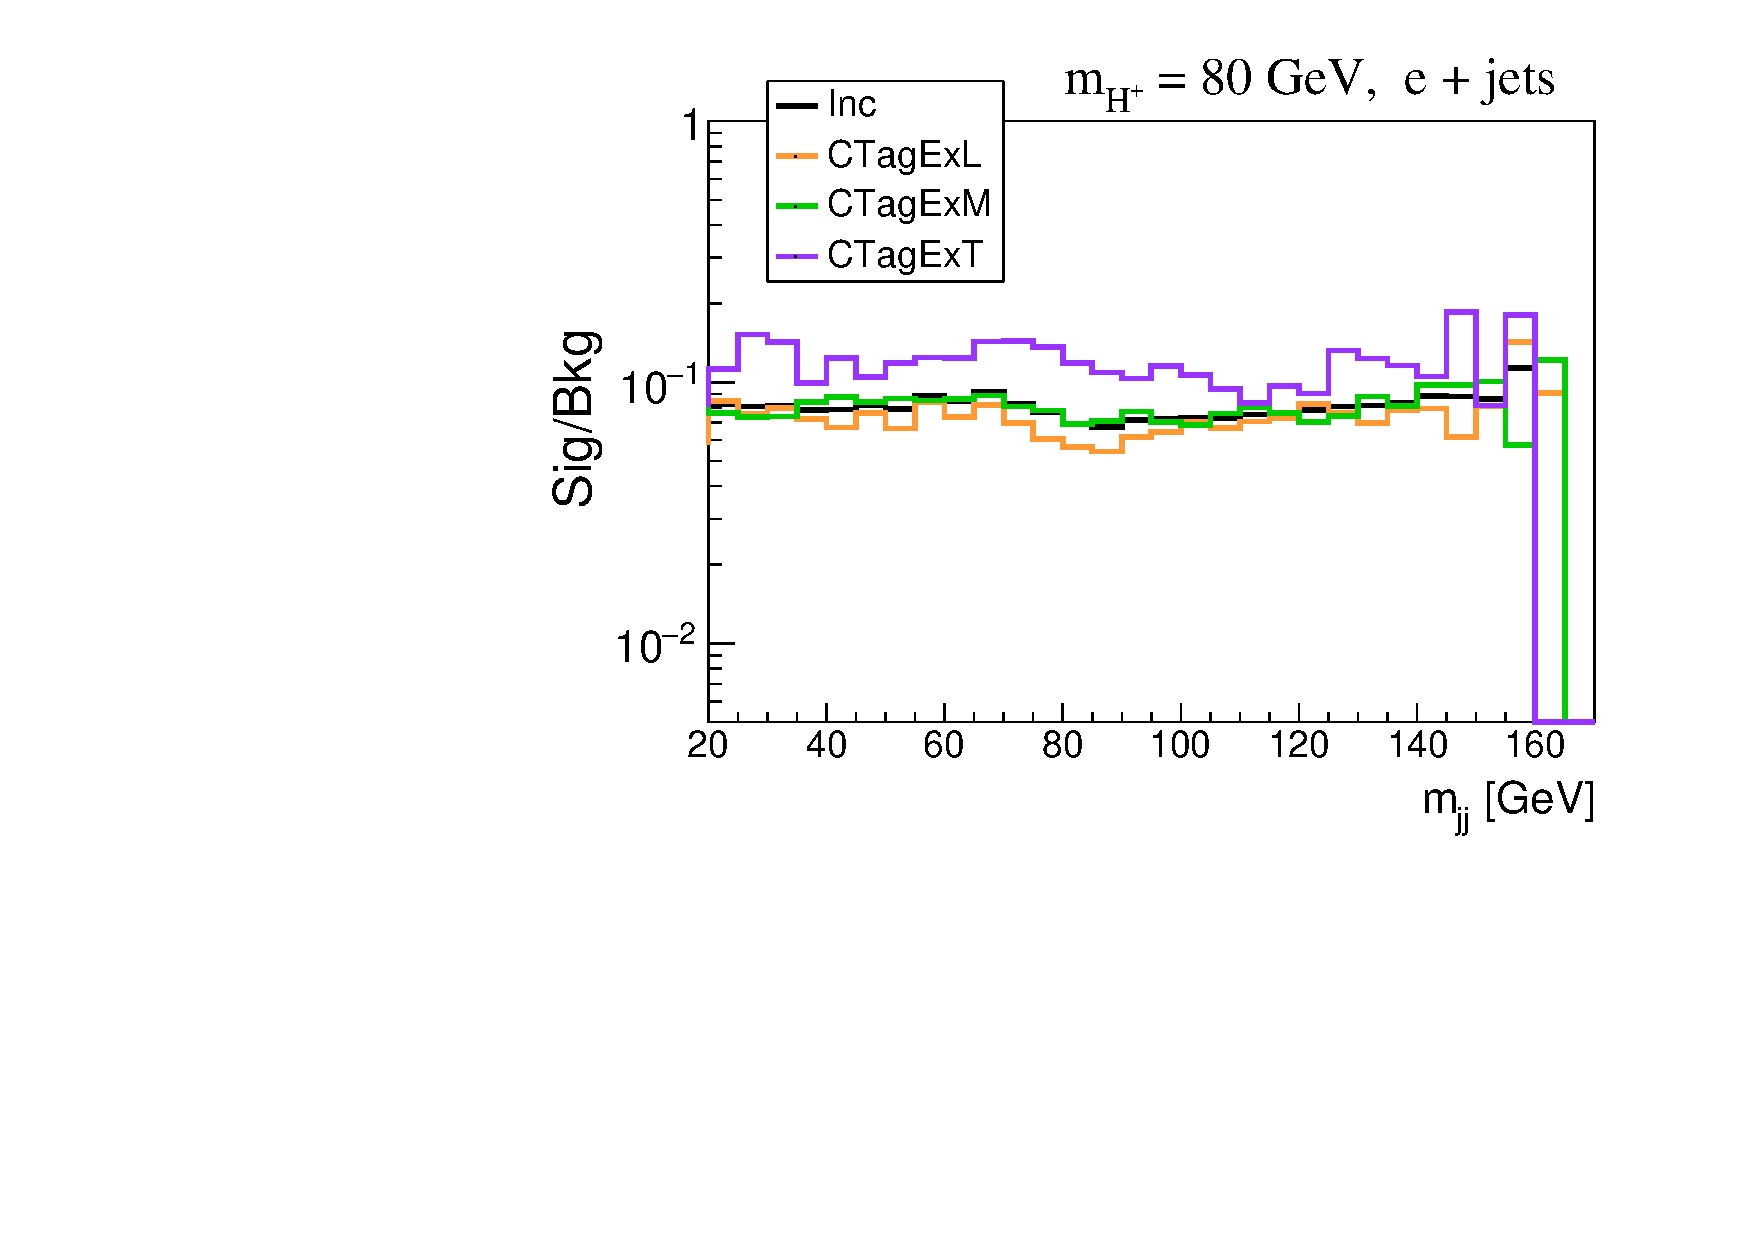
\includegraphics[width=0.40\linewidth]{Image/Electron/CTag/WH80_ele_ratioSB.pdf}}
\vfil
\subfigure[]{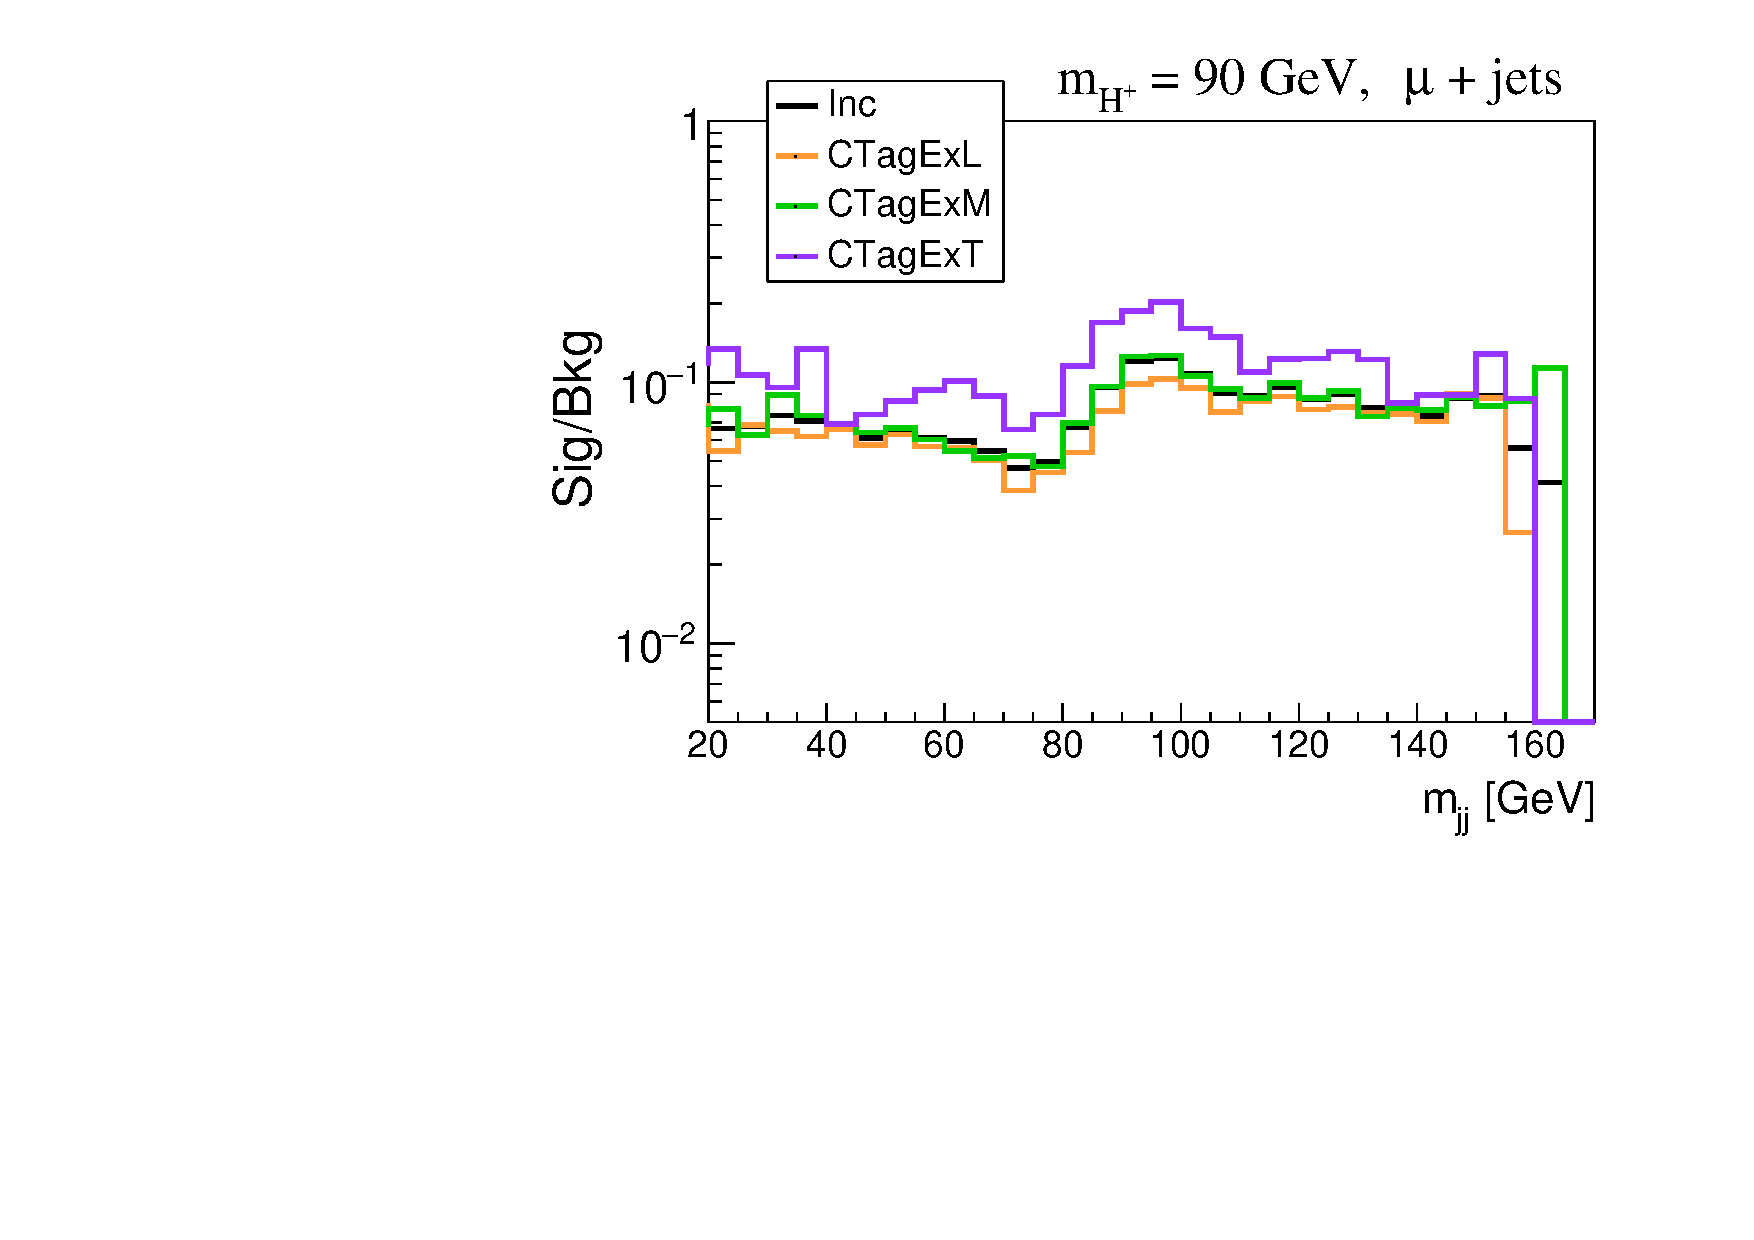
\includegraphics[width=0.40\linewidth]{Image/Muon/CTag/WH90_mu_ratioSB.pdf}}
\subfigure[]{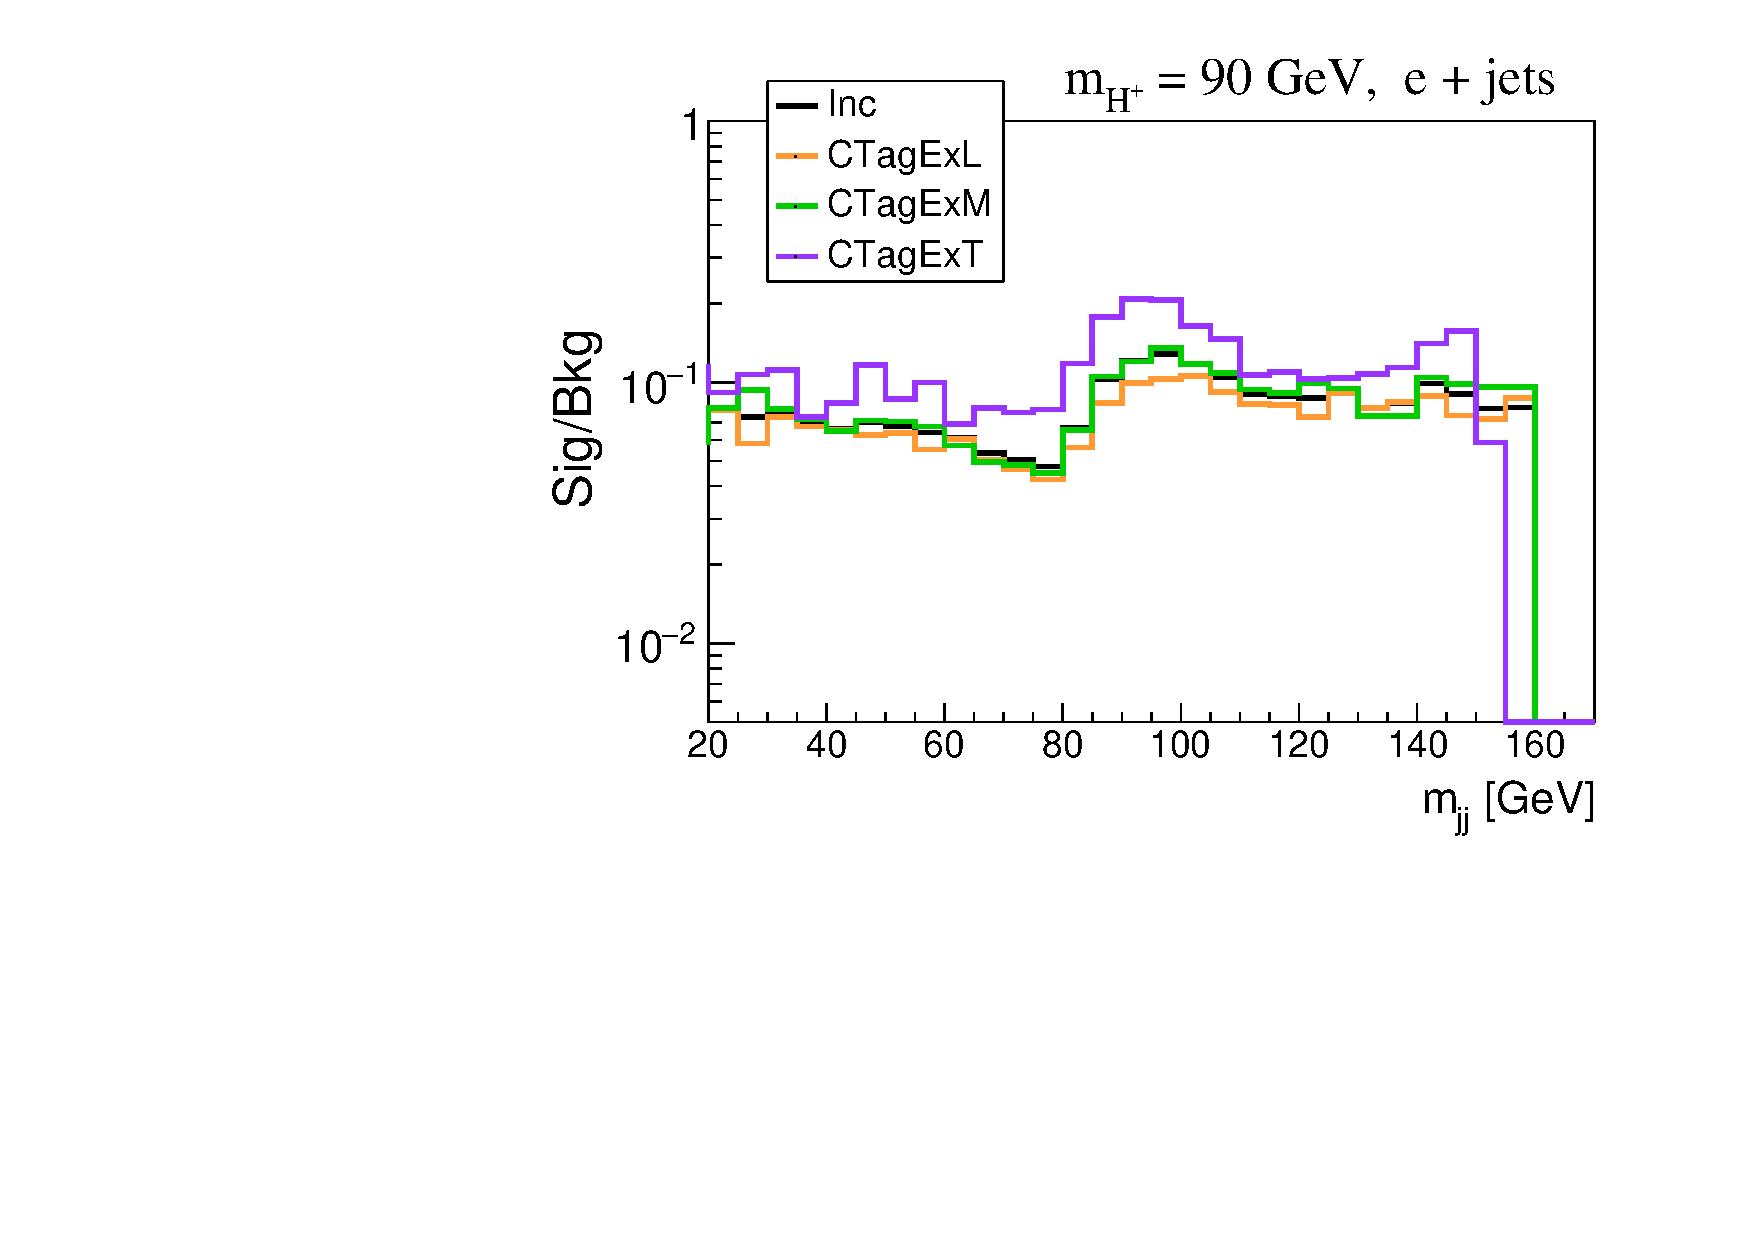
\includegraphics[width=0.40\linewidth]{Image/Electron/CTag/WH90_ele_ratioSB.pdf}}
\vfil
\subfigure[]{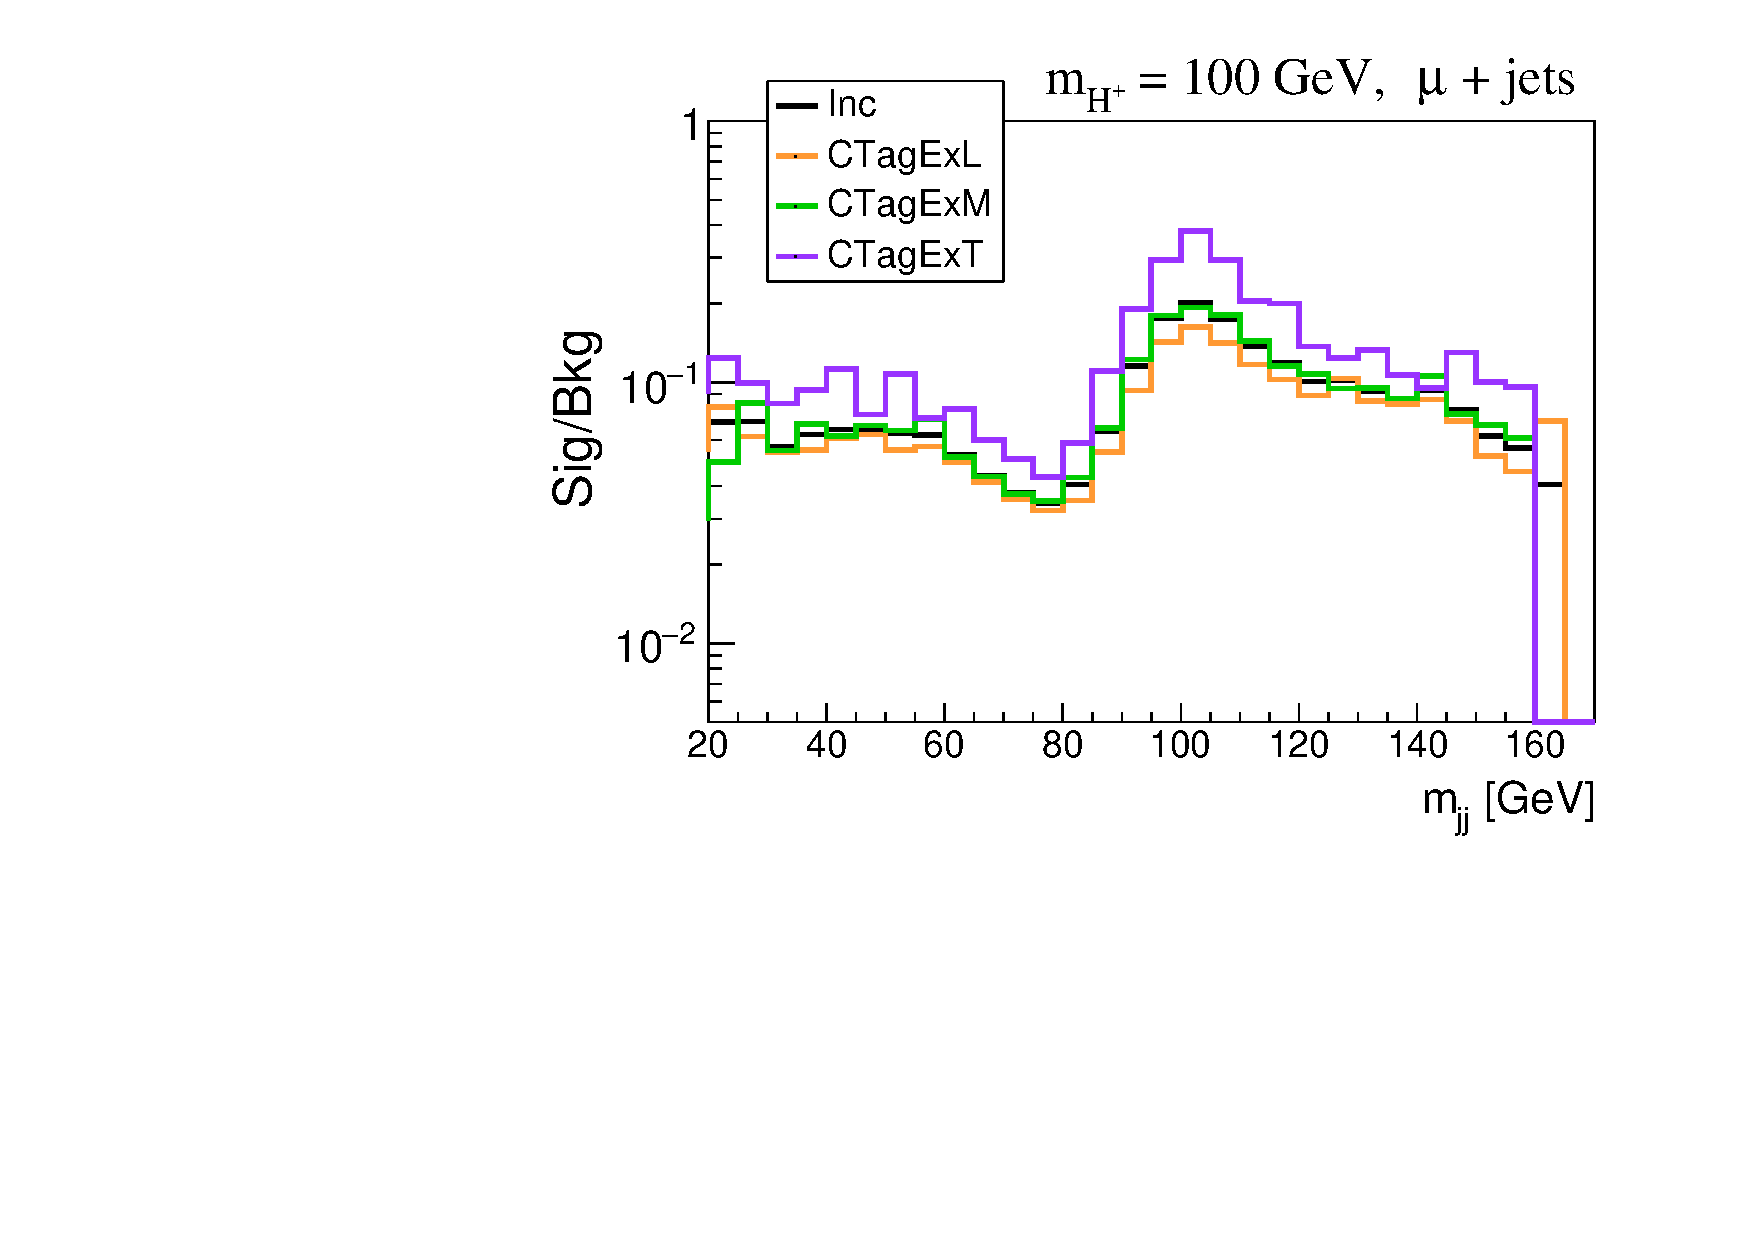
\includegraphics[width=0.40\linewidth]{Image/Muon/CTag/WH100_mu_ratioSB.pdf}}
\subfigure[]{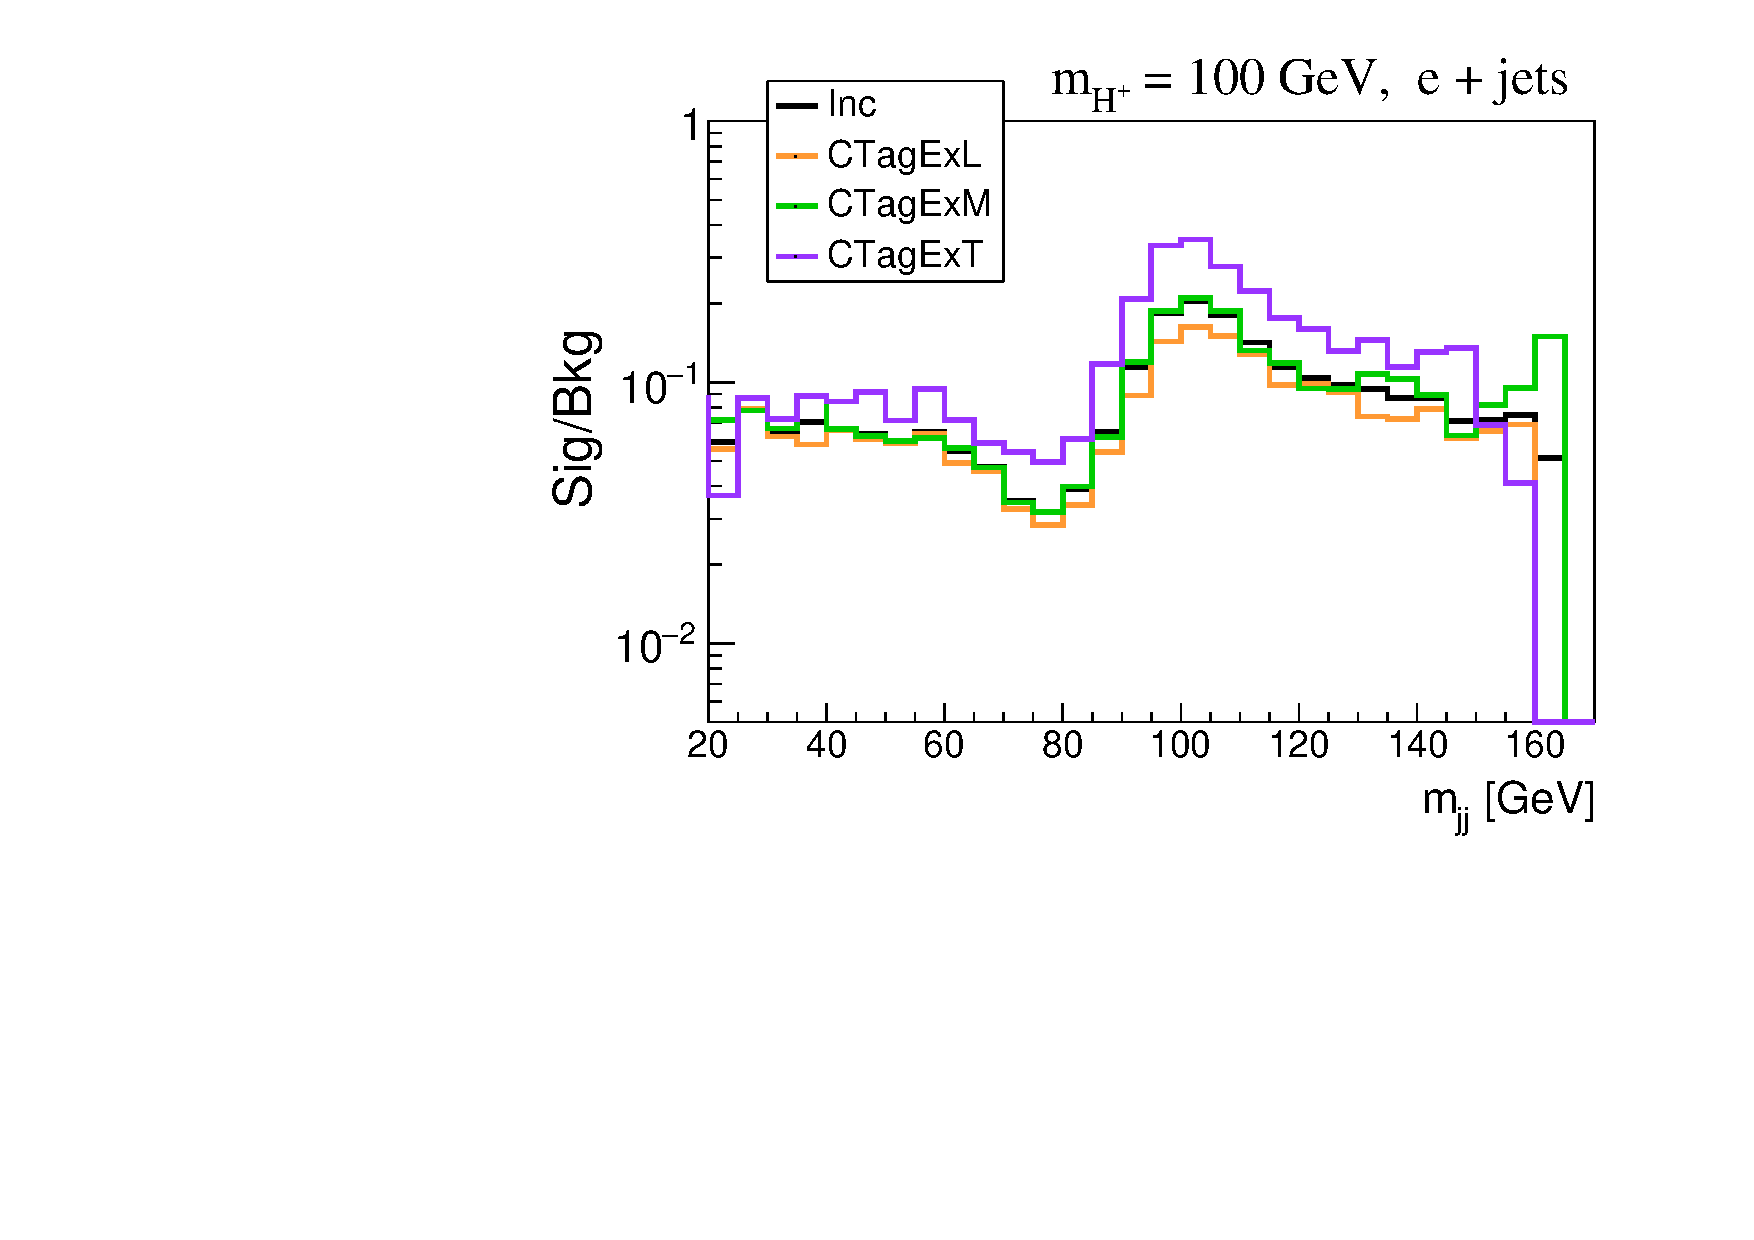
\includegraphics[width=0.40\linewidth]{Image/Electron/CTag/WH100_ele_ratioSB.pdf}}
\vfil
\subfigure[]{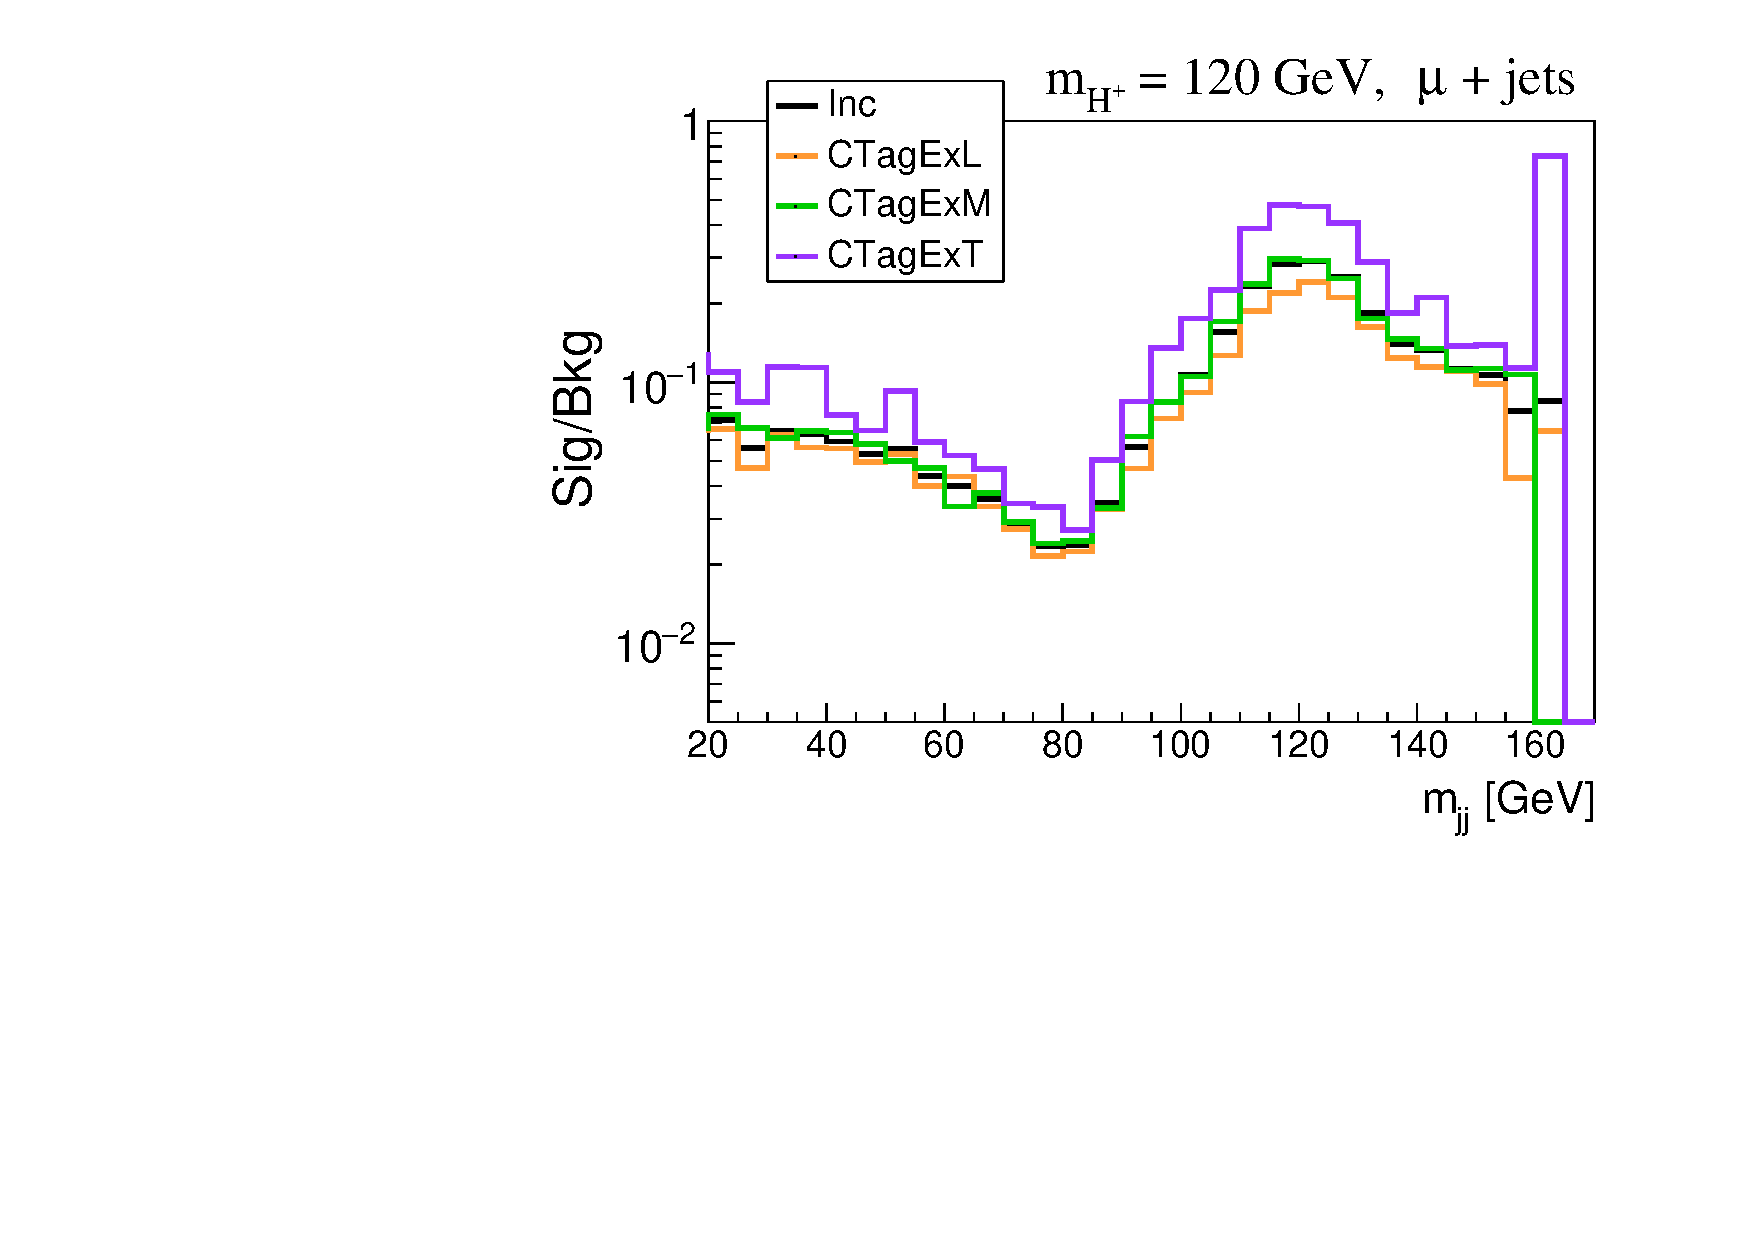
\includegraphics[width=0.40\linewidth]{Image/Muon/CTag/WH120_mu_ratioSB.pdf}}
\subfigure[]{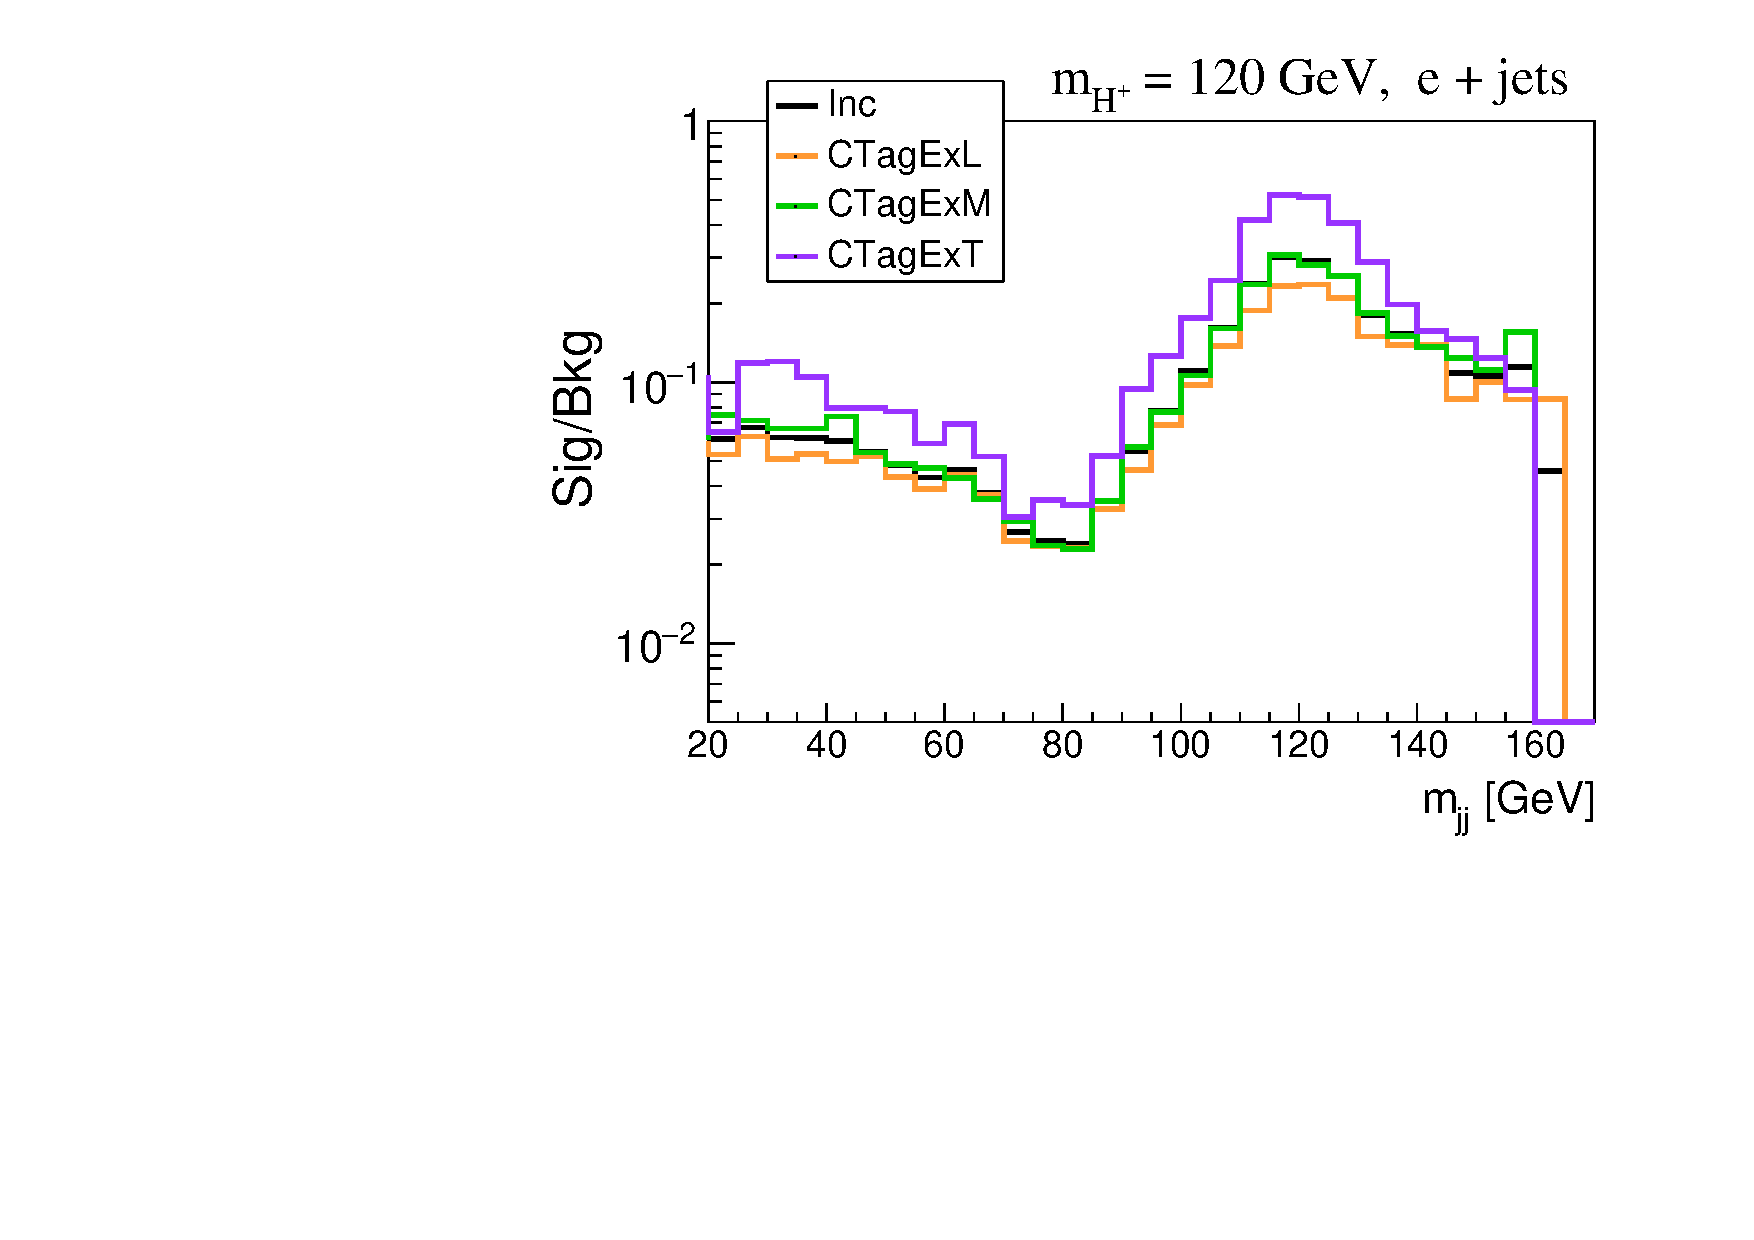
\includegraphics[width=0.40\linewidth]{Image/Electron/CTag/WH120_ele_ratioSB.pdf}}
\caption{Signal to background ratio for $\mHp$ = 80, 90, 100, 120 \GeV.}
\label{fig:ratioSB_1}
\end{figure}

\begin{figure}
\centering  
\subfigure[]{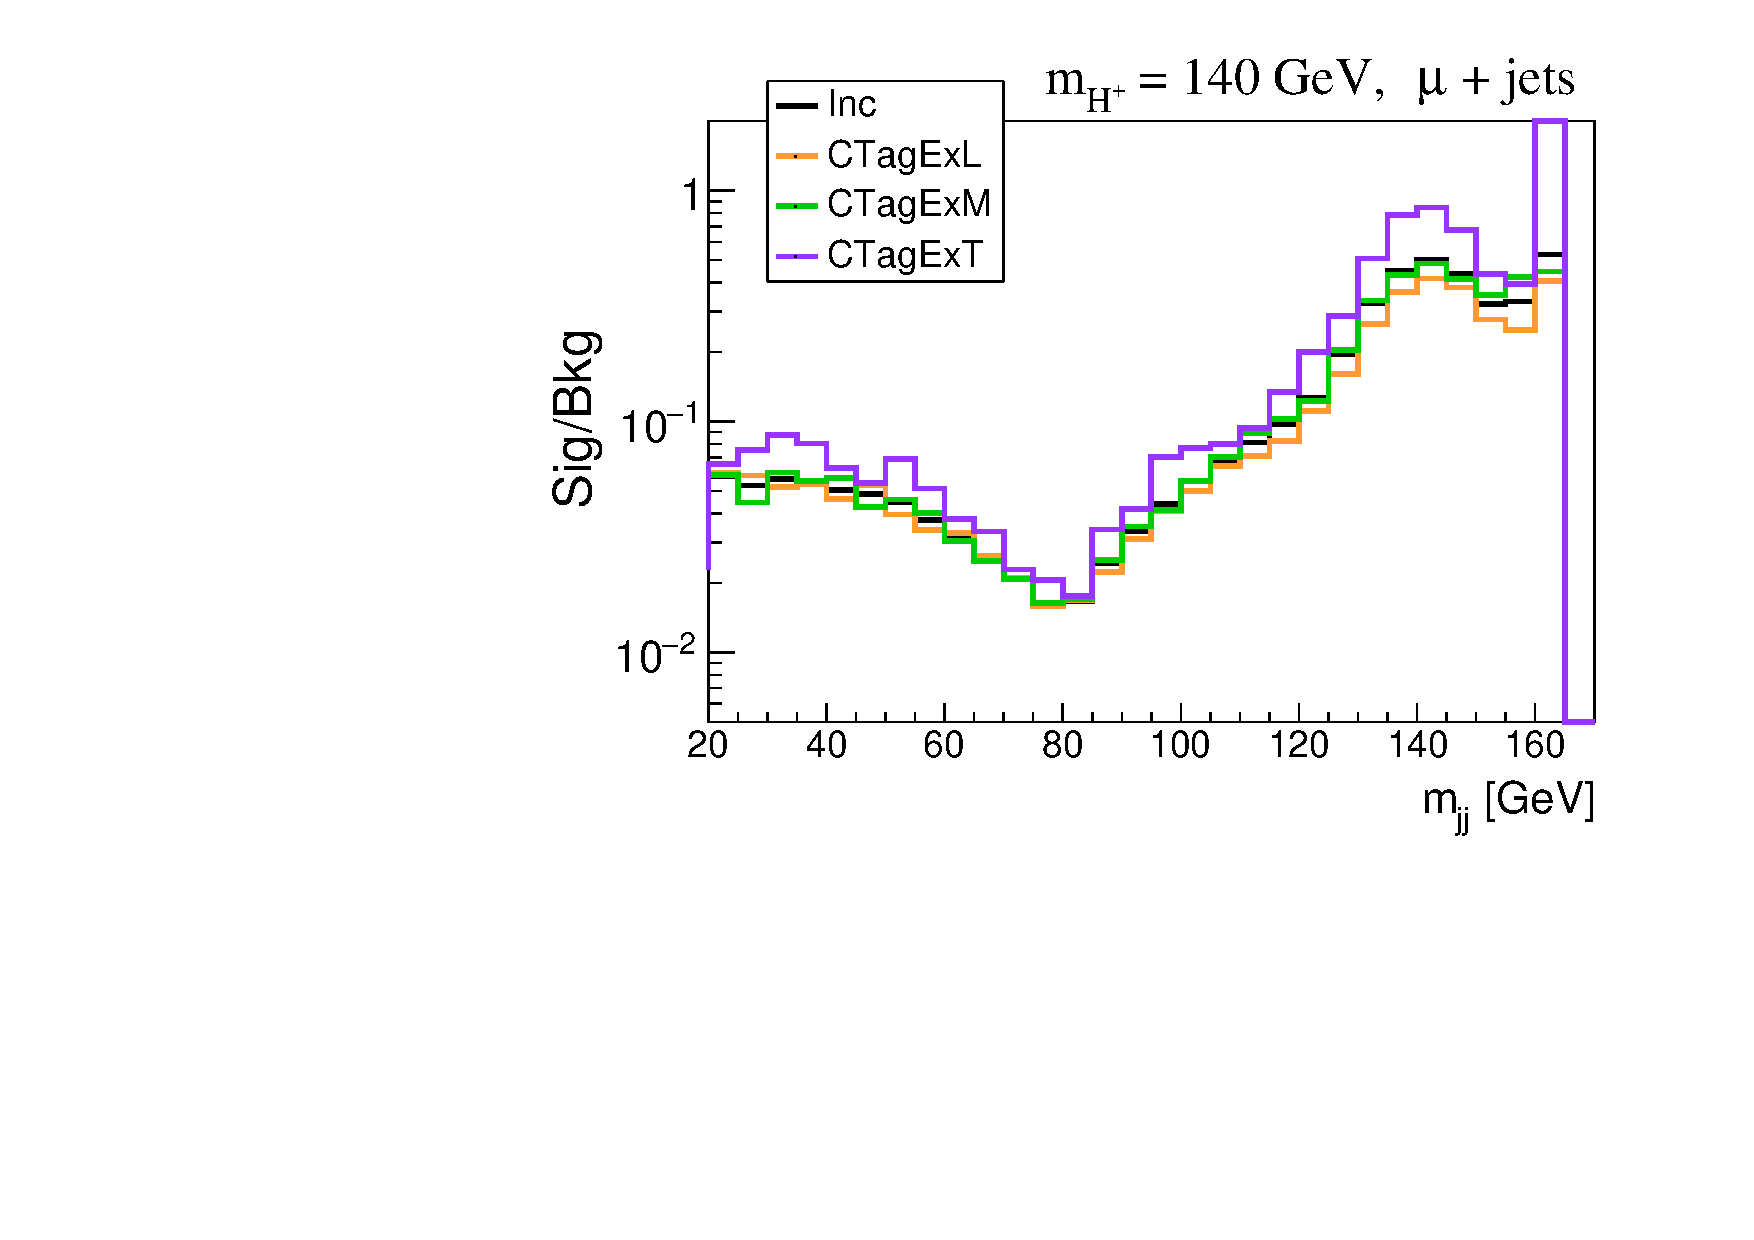
\includegraphics[width=0.40\linewidth]{Image/Muon/CTag/WH140_mu_ratioSB.pdf}}
\subfigure[]{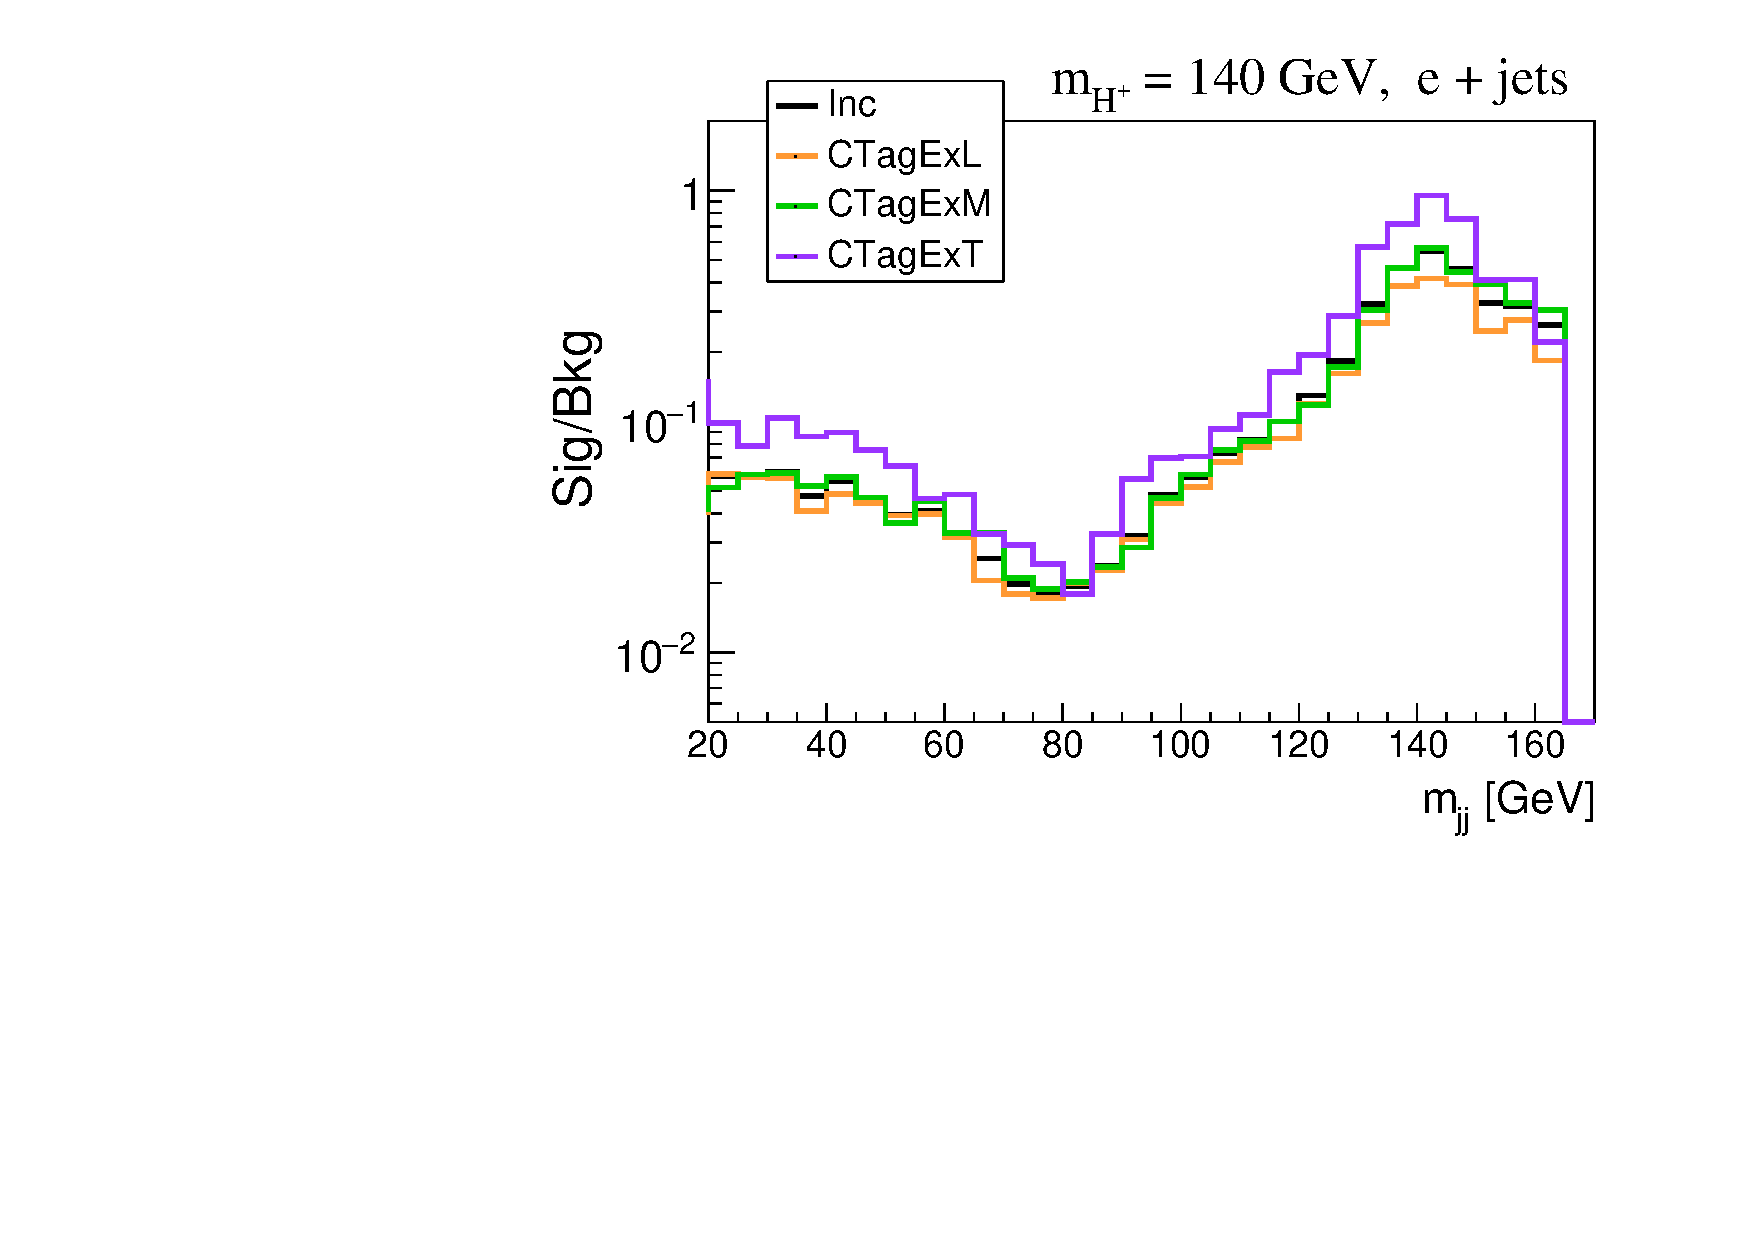
\includegraphics[width=0.40\linewidth]{Image/Electron/CTag/WH140_ele_ratioSB.pdf}}
\vfil
\subfigure[]{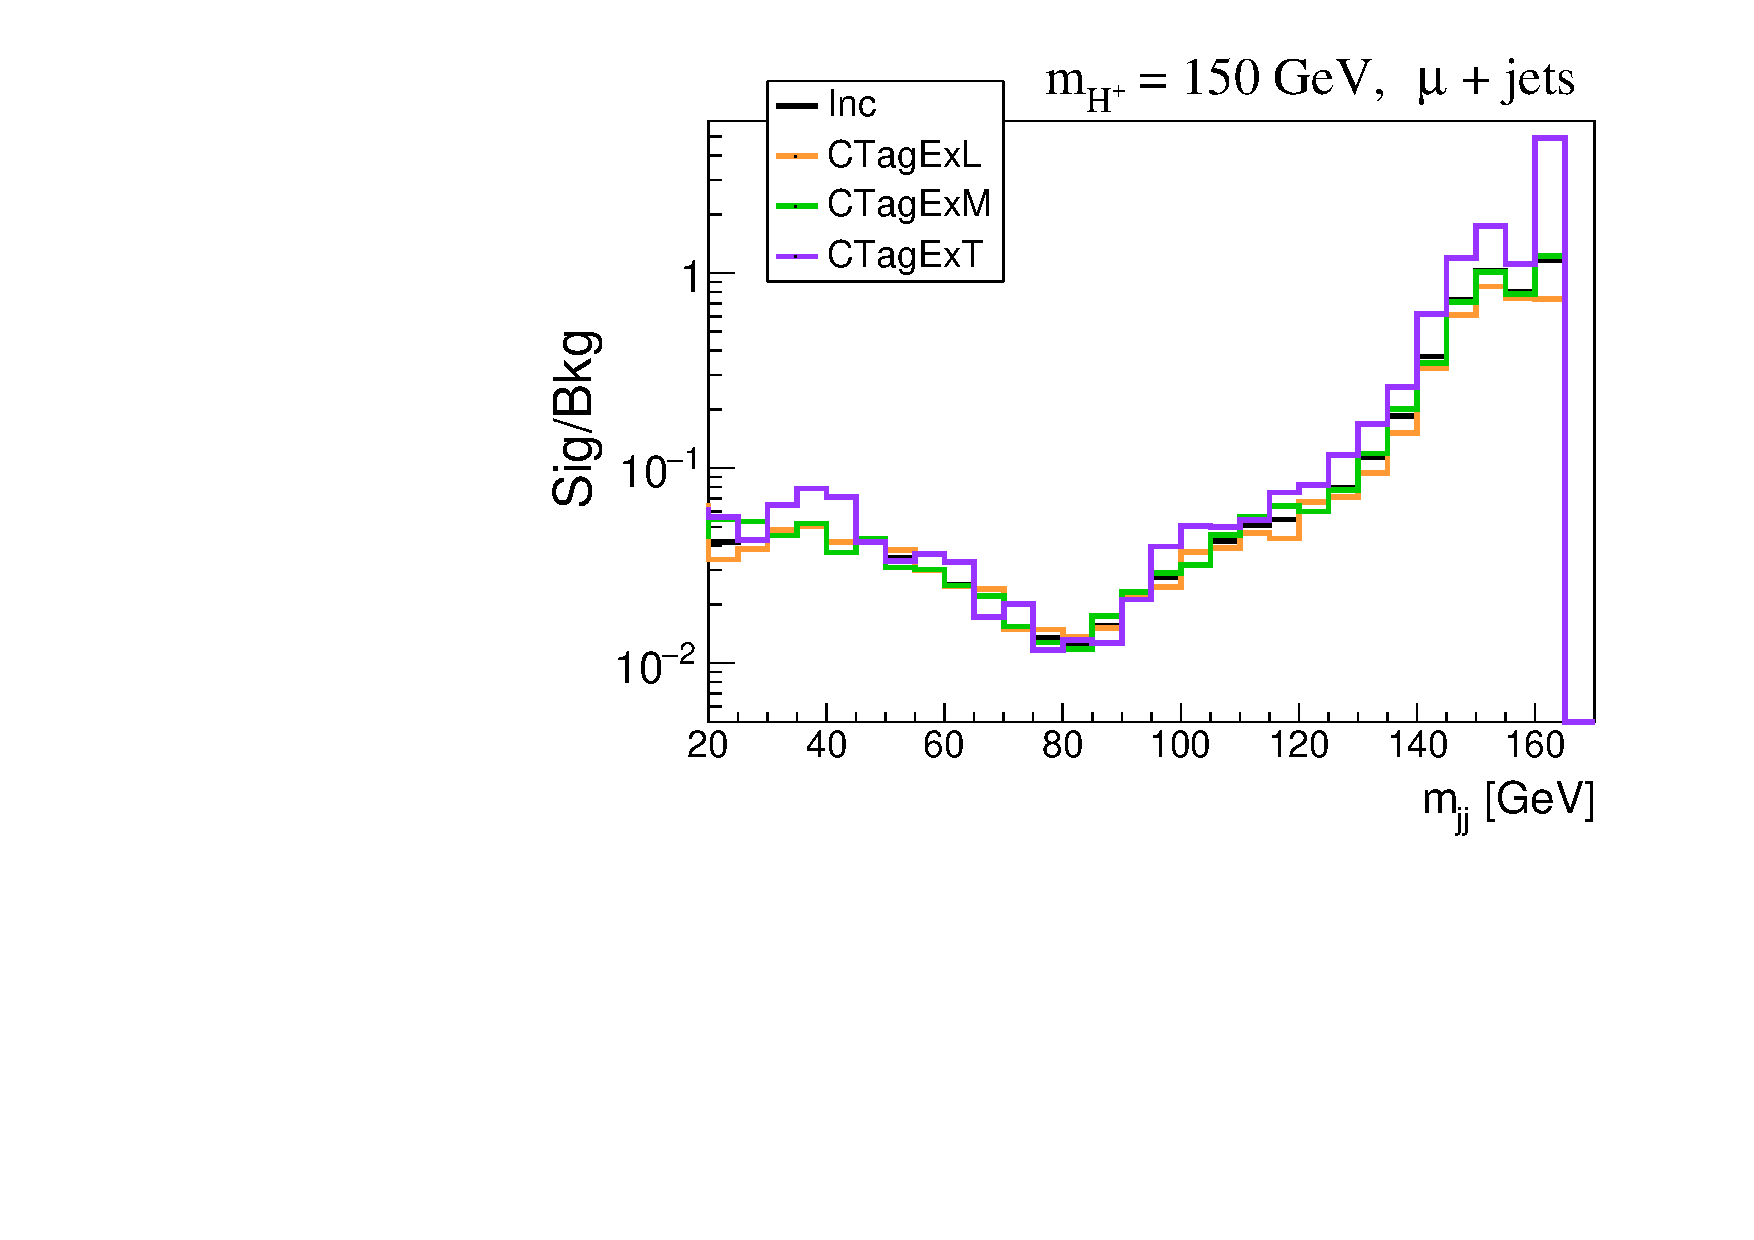
\includegraphics[width=0.40\linewidth]{Image/Muon/CTag/WH150_mu_ratioSB.pdf}}
\subfigure[]{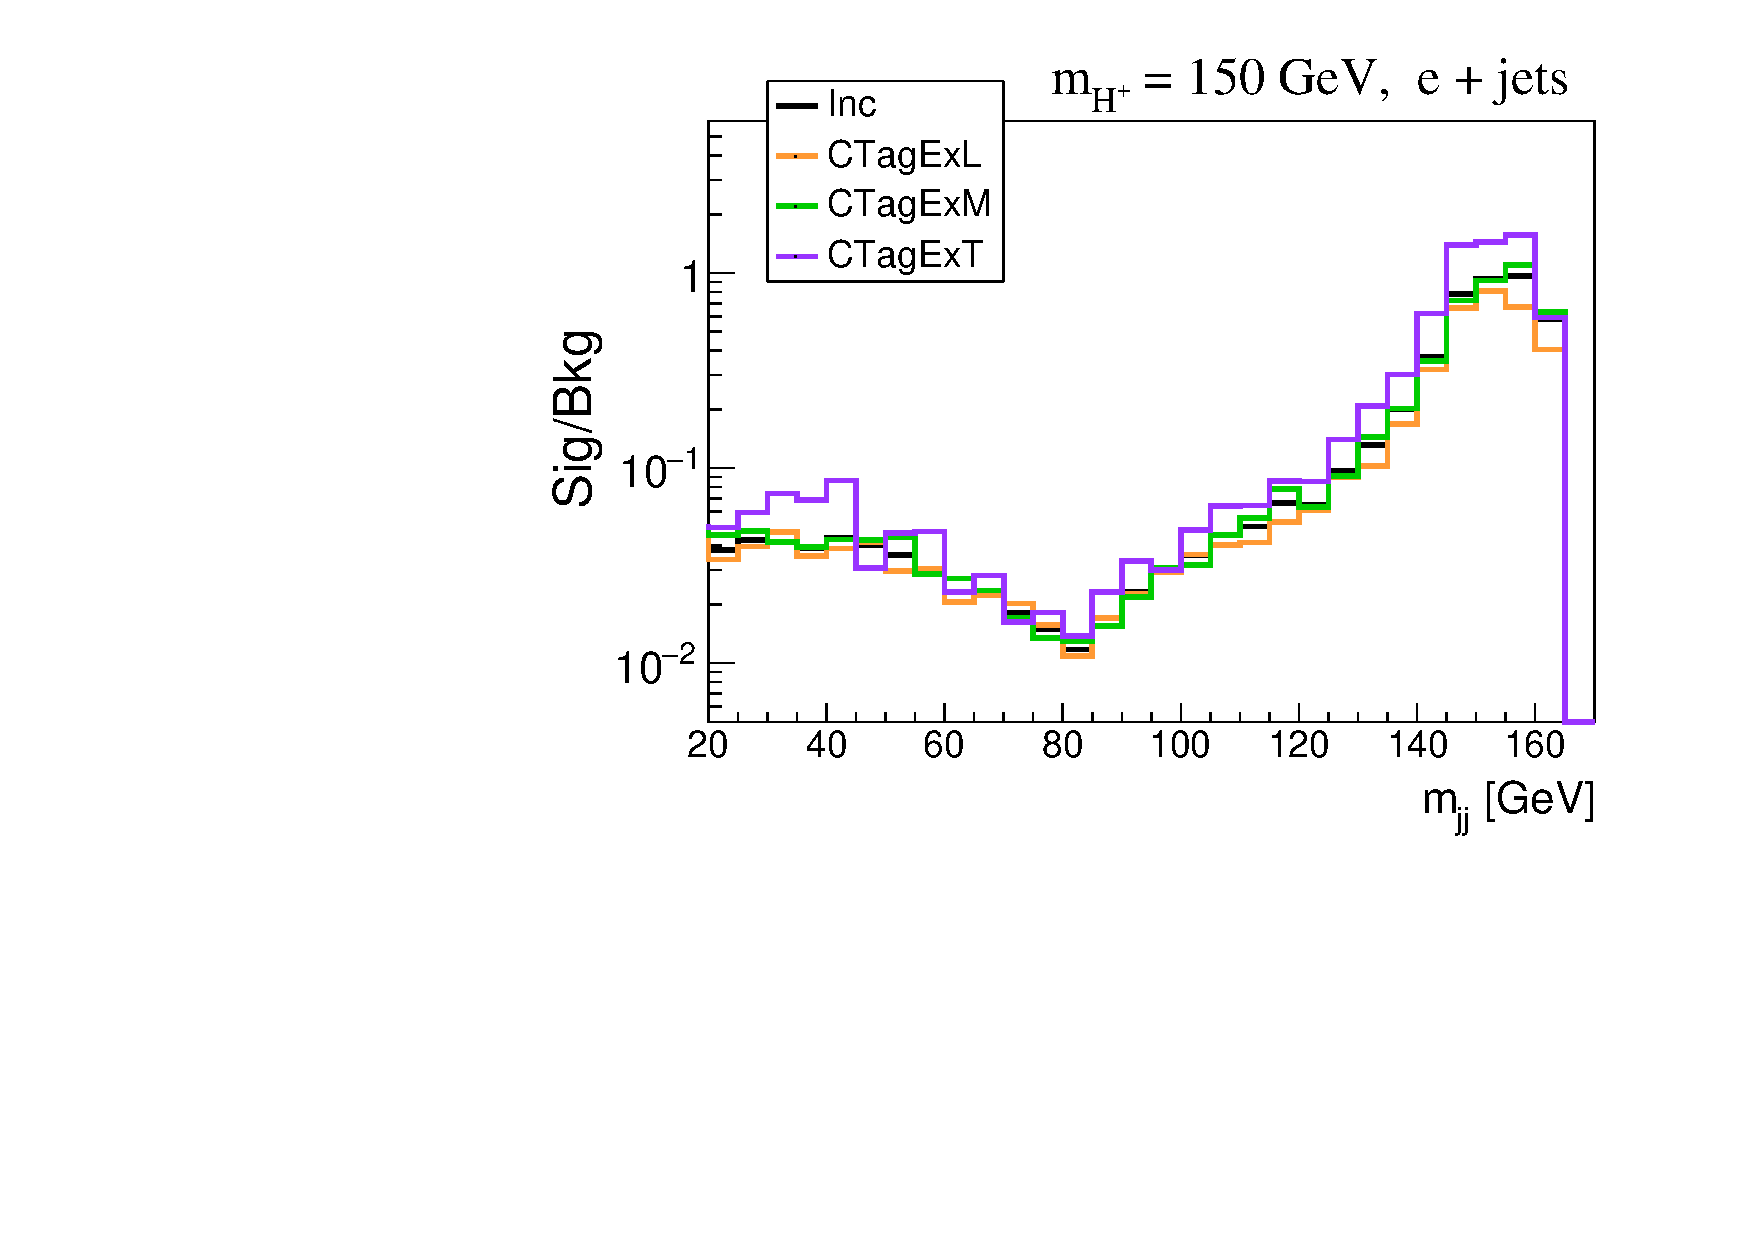
\includegraphics[width=0.40\linewidth]{Image/Electron/CTag/WH150_ele_ratioSB.pdf}}
\vfil
\subfigure[]{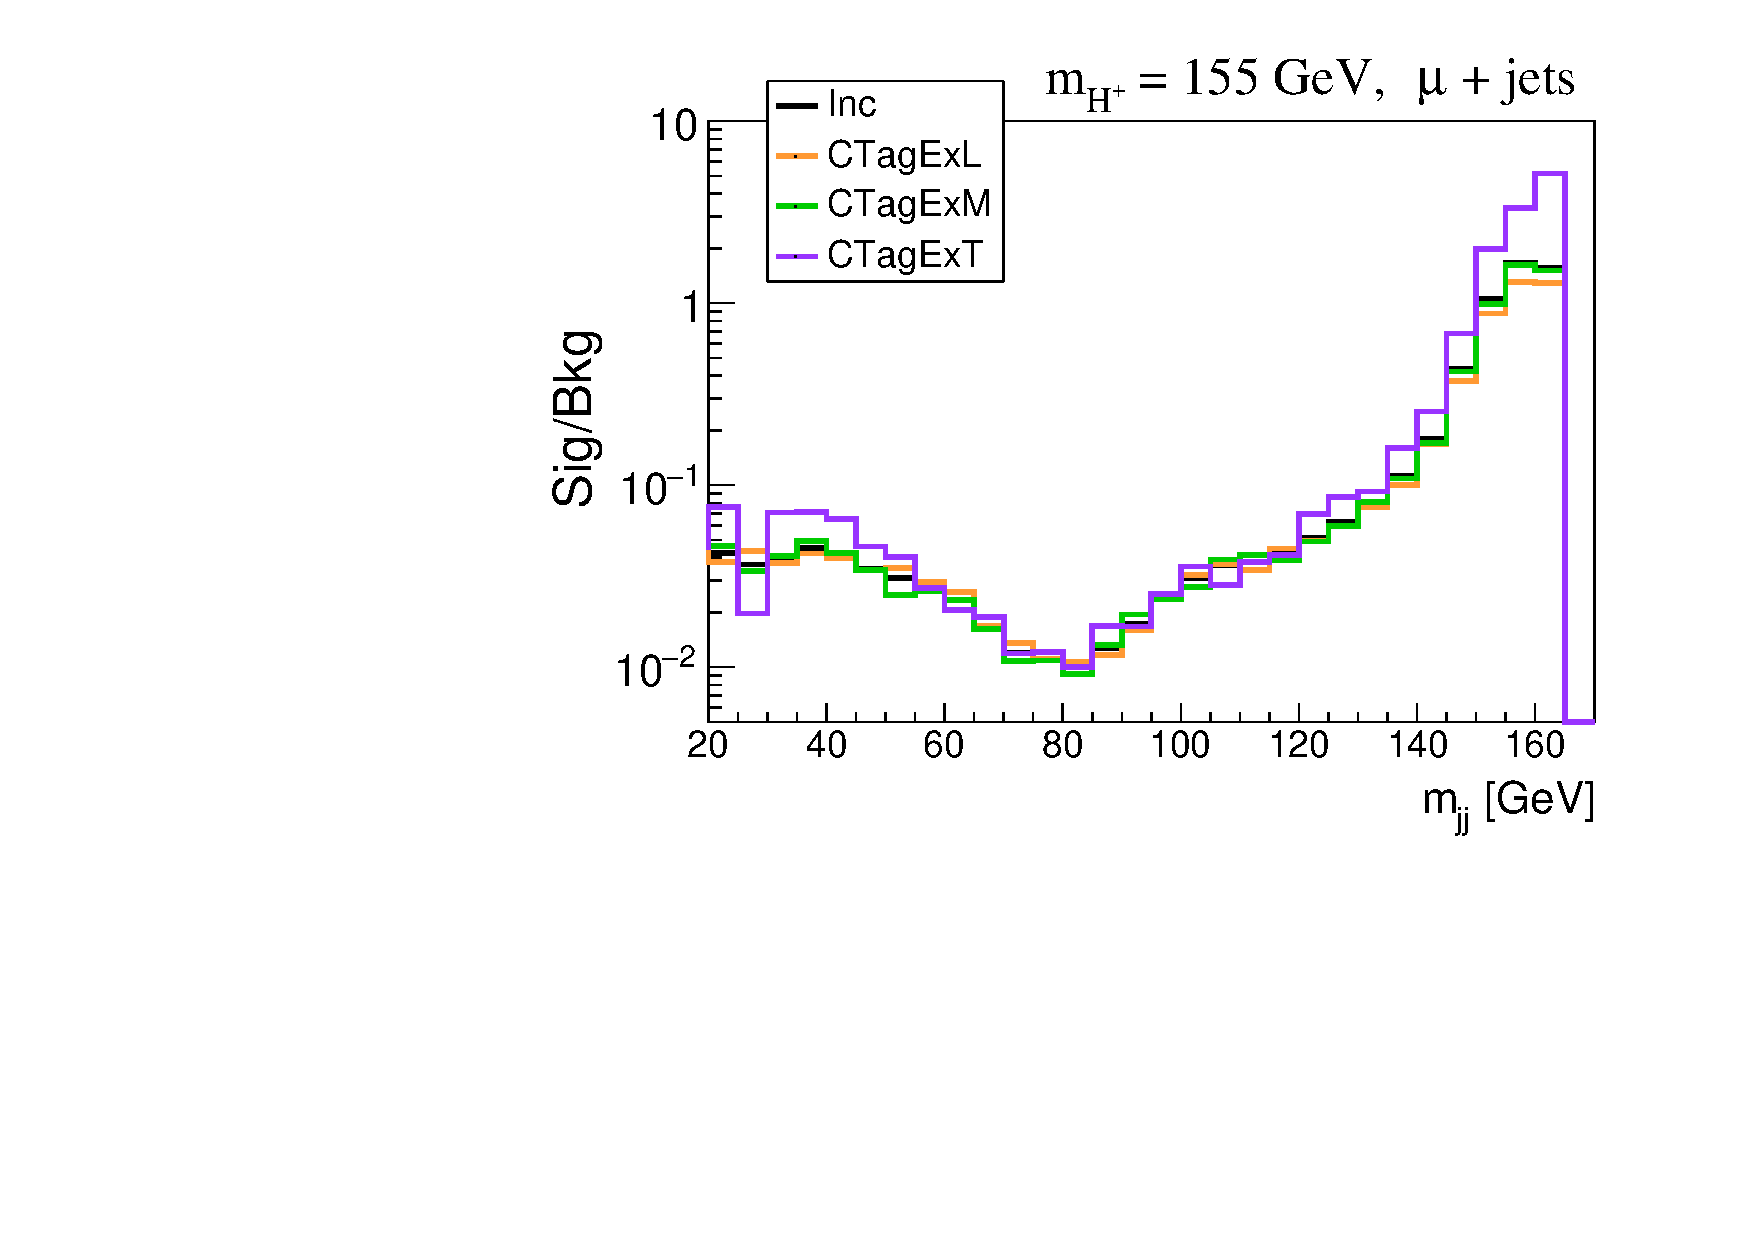
\includegraphics[width=0.40\linewidth]{Image/Muon/CTag/WH155_mu_ratioSB.pdf}}
\subfigure[]{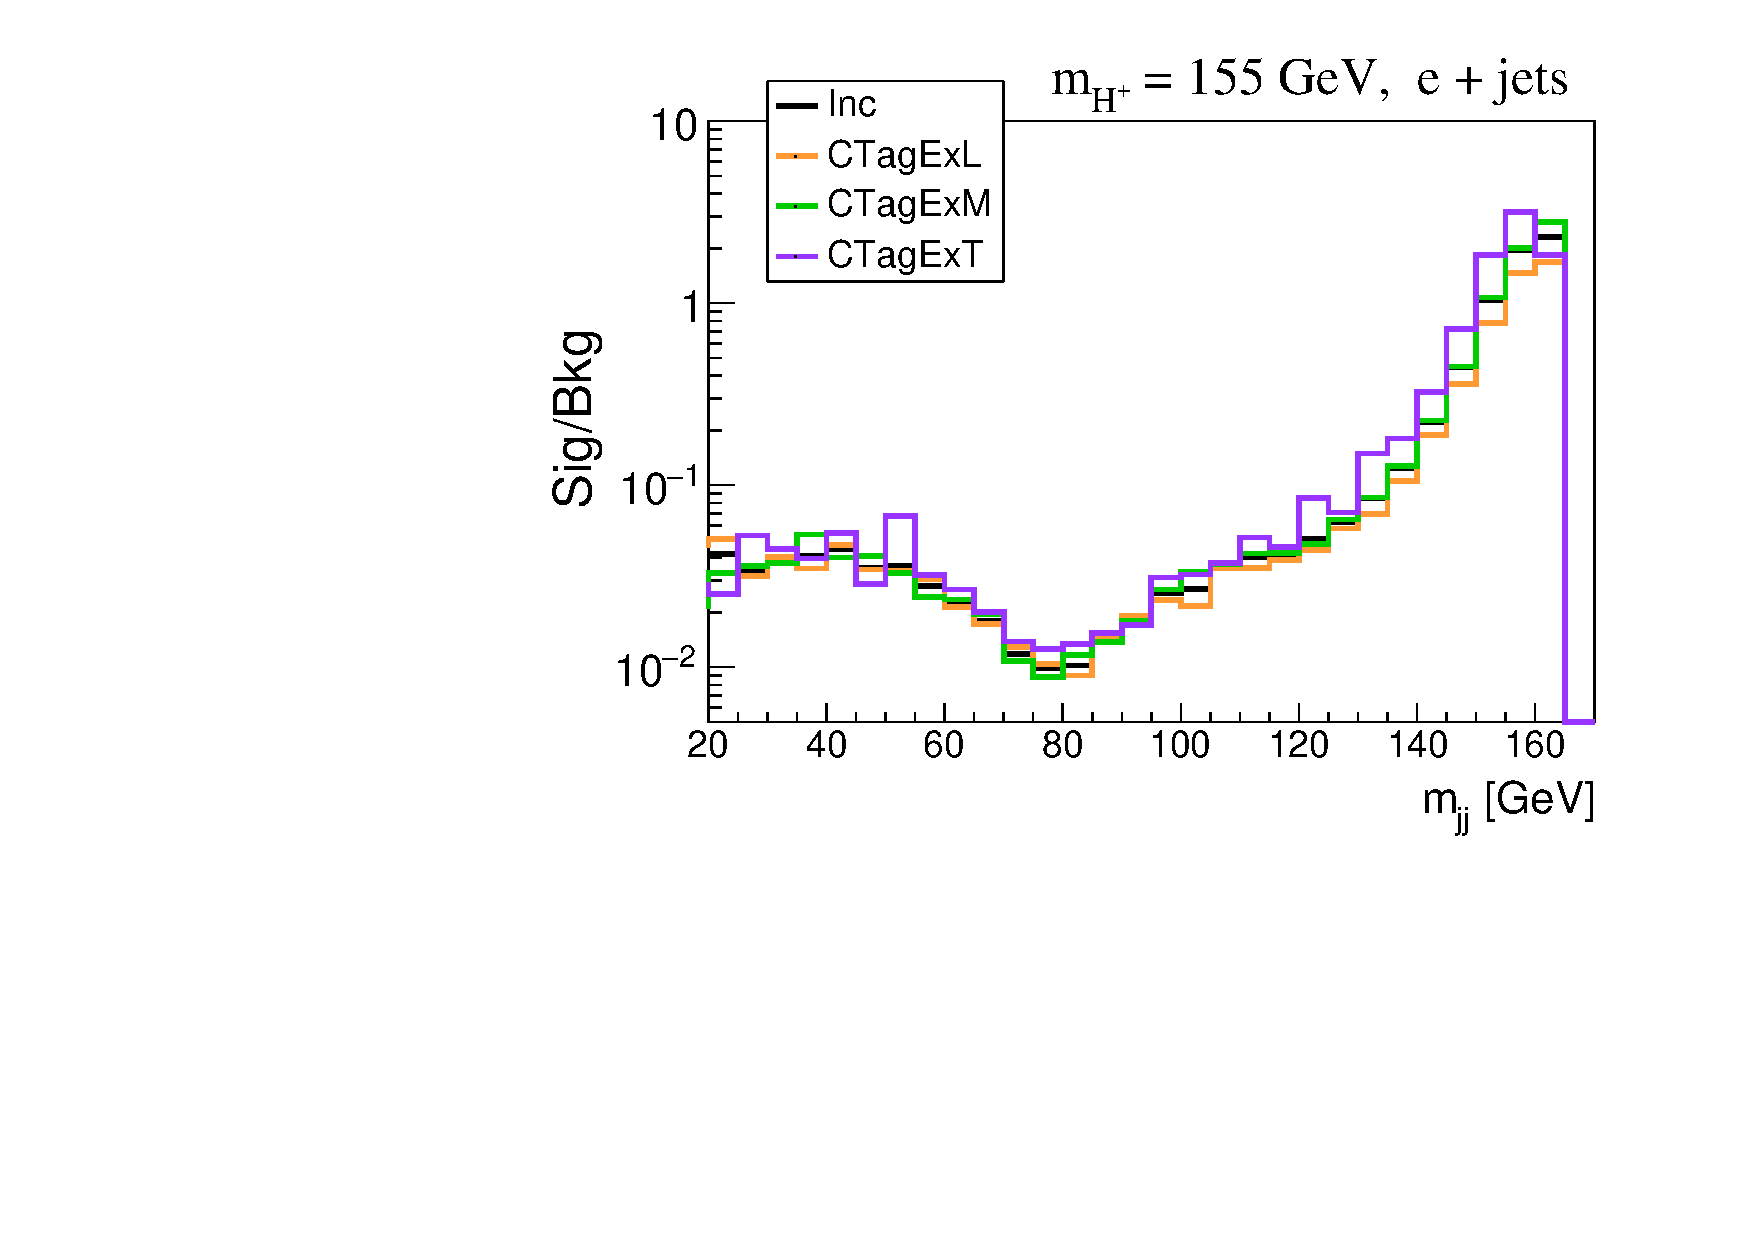
\includegraphics[width=0.40\linewidth]{Image/Electron/CTag/WH155_ele_ratioSB.pdf}}
\vfil
\subfigure[]{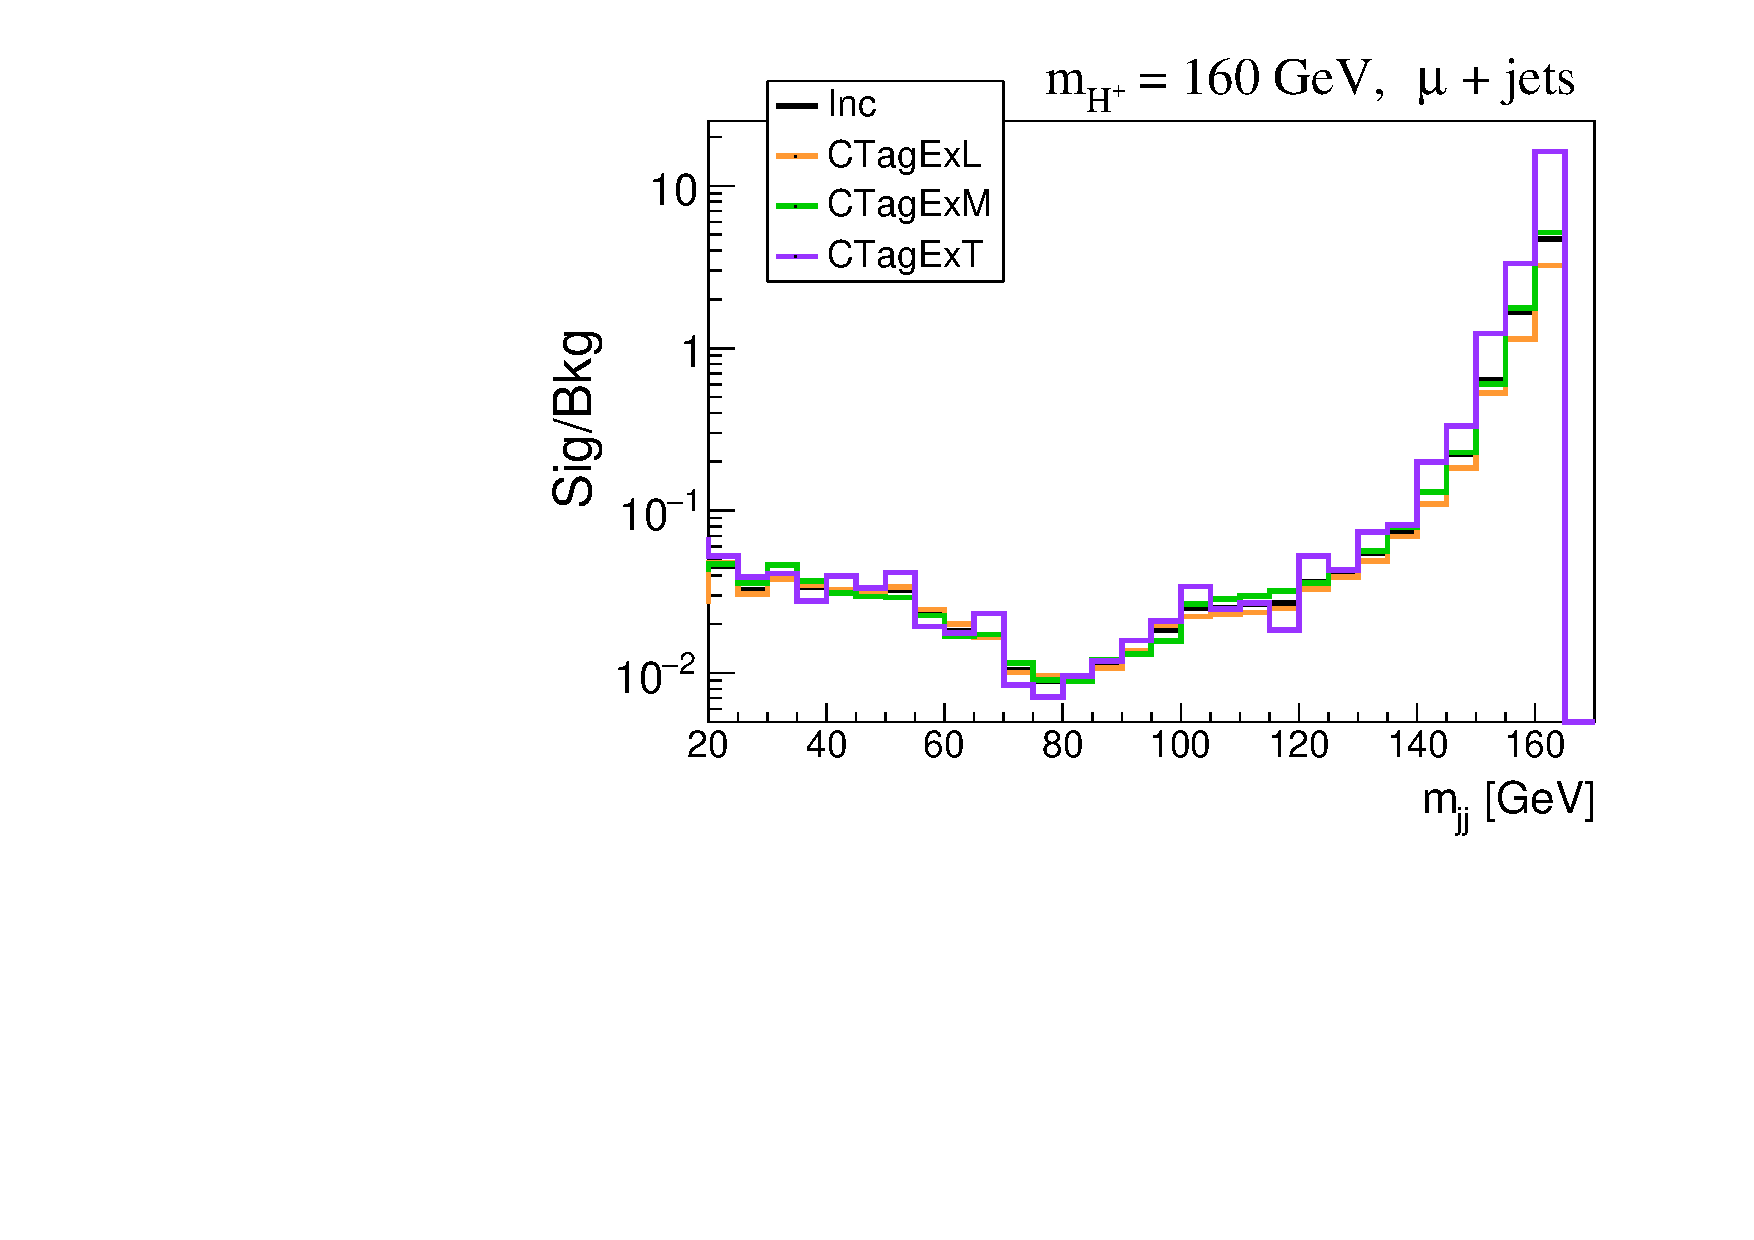
\includegraphics[width=0.40\linewidth]{Image/Muon/CTag/WH160_mu_ratioSB.pdf}}
\subfigure[]{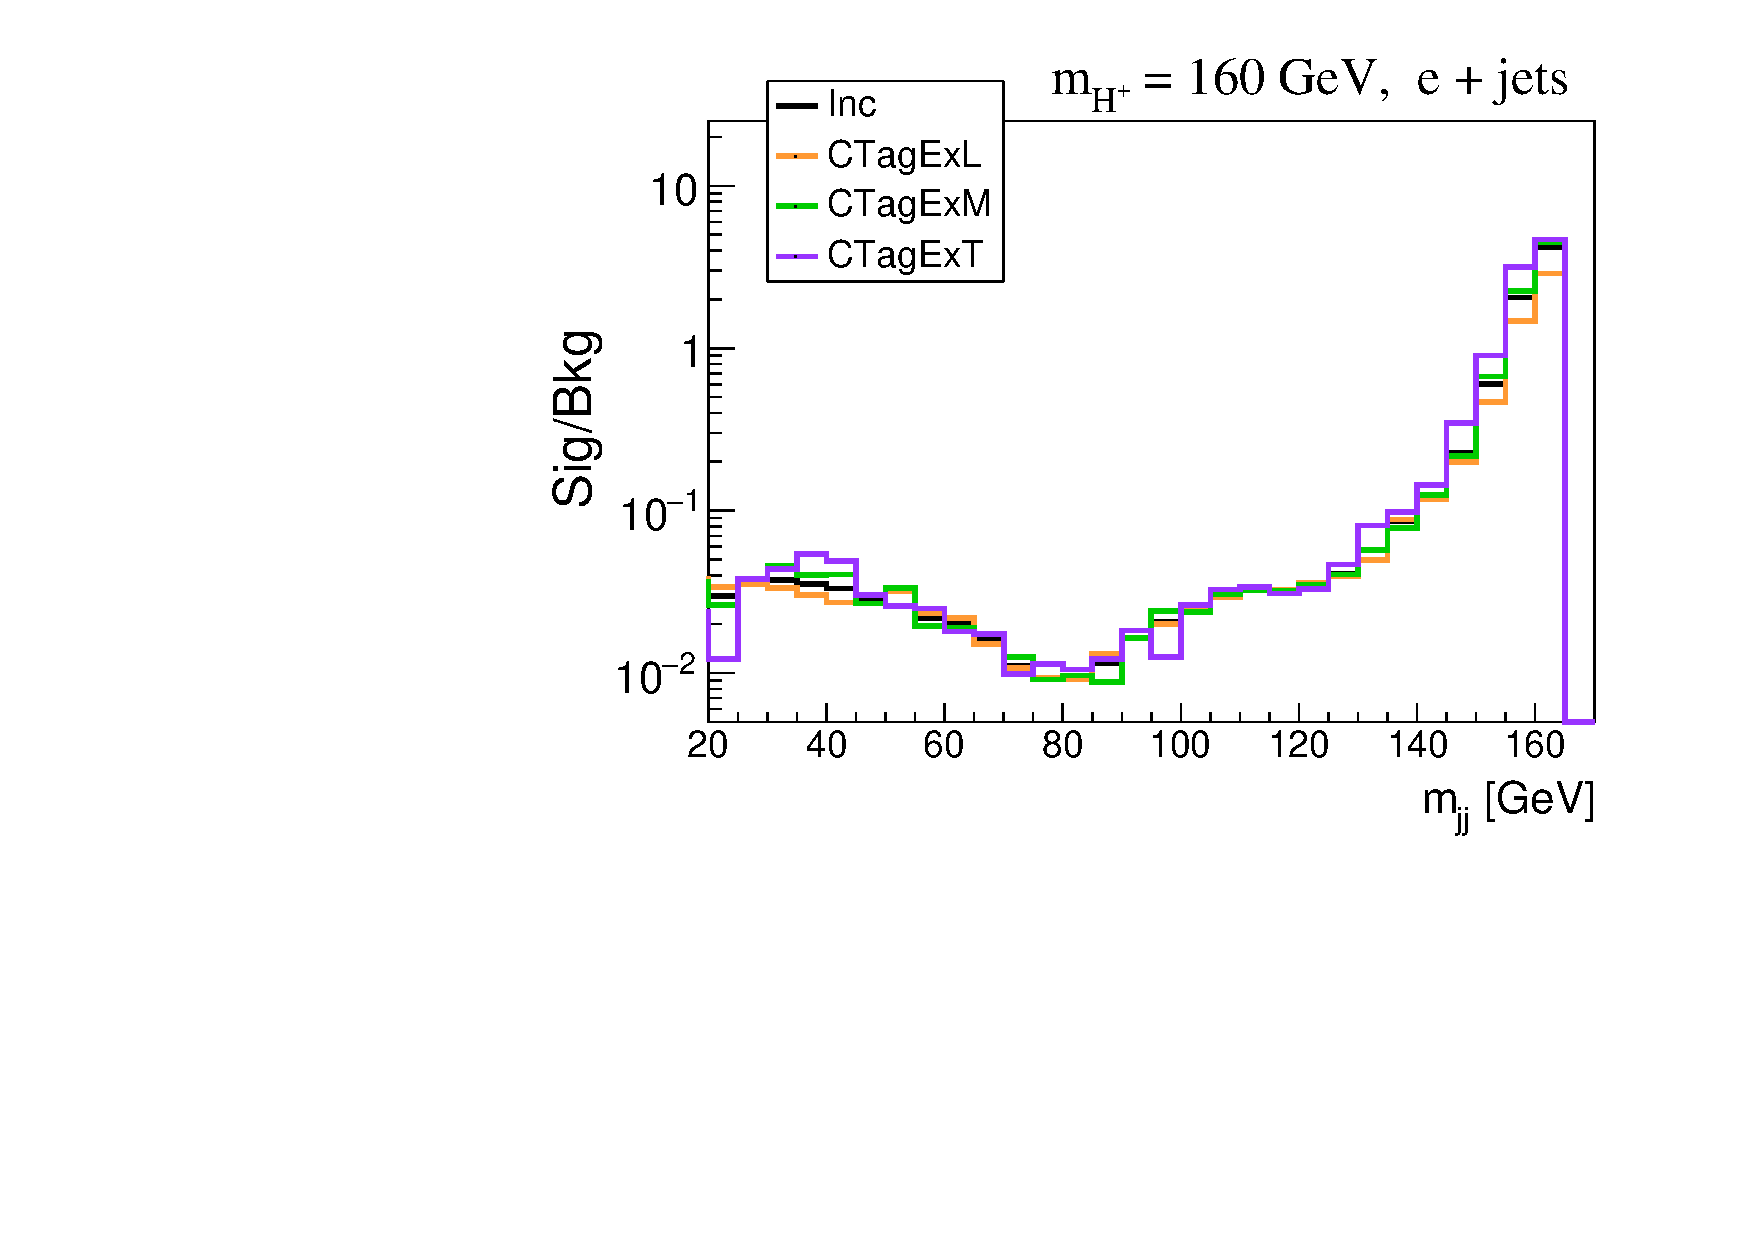
\includegraphics[width=0.40\linewidth]{Image/Electron/CTag/WH160_ele_ratioSB.pdf}}
\caption{Signal to background ratio for $\mHp$ = 140, 150, 155, 160 \GeV.}
\label{fig:ratioSB_2}
\end{figure}

\begin{figure}
\begin{center}
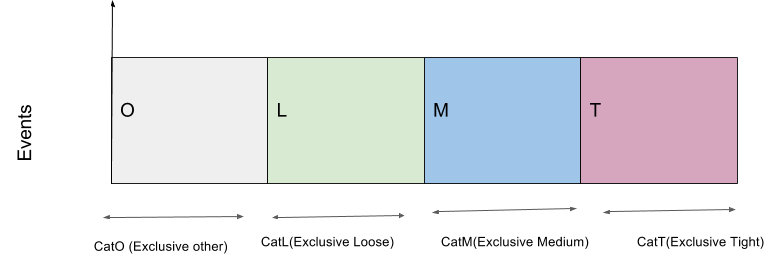
\includegraphics[width=1.00\textwidth]{Image/Limit/cTagCat.png}
\caption{Exclusive event categories based on different charm tagging. The events falling
in the exclusive \dq{other} category are not considered in this analysis. However, fraction of
events falling in this category is very small.}
\label{fig:cTagCat}
\end{center}
\end{figure}
The $\mjj$ distribution from exclusive charm categories is shown in 
Figure~\ref{fig:mjj_cTagEx}. The corresponding event yields are shown in 
Table~\ref{tab:eventYieldCTagEx}. The signal to background ratio is 
shown in Figures~\ref{fig:ratioSB_1},~\ref{fig:ratioSB_2} for different masses 
of charged Higgs for both channels. From these figures, one can see that the 
signal to background ratio is different in different categories. The \mjj distributions
from these three categories are combined to compute limits as described in 
Section~\ref{ss:limit_cTagEx}.
\begin{figure}
\centering  
\subfigure[]
{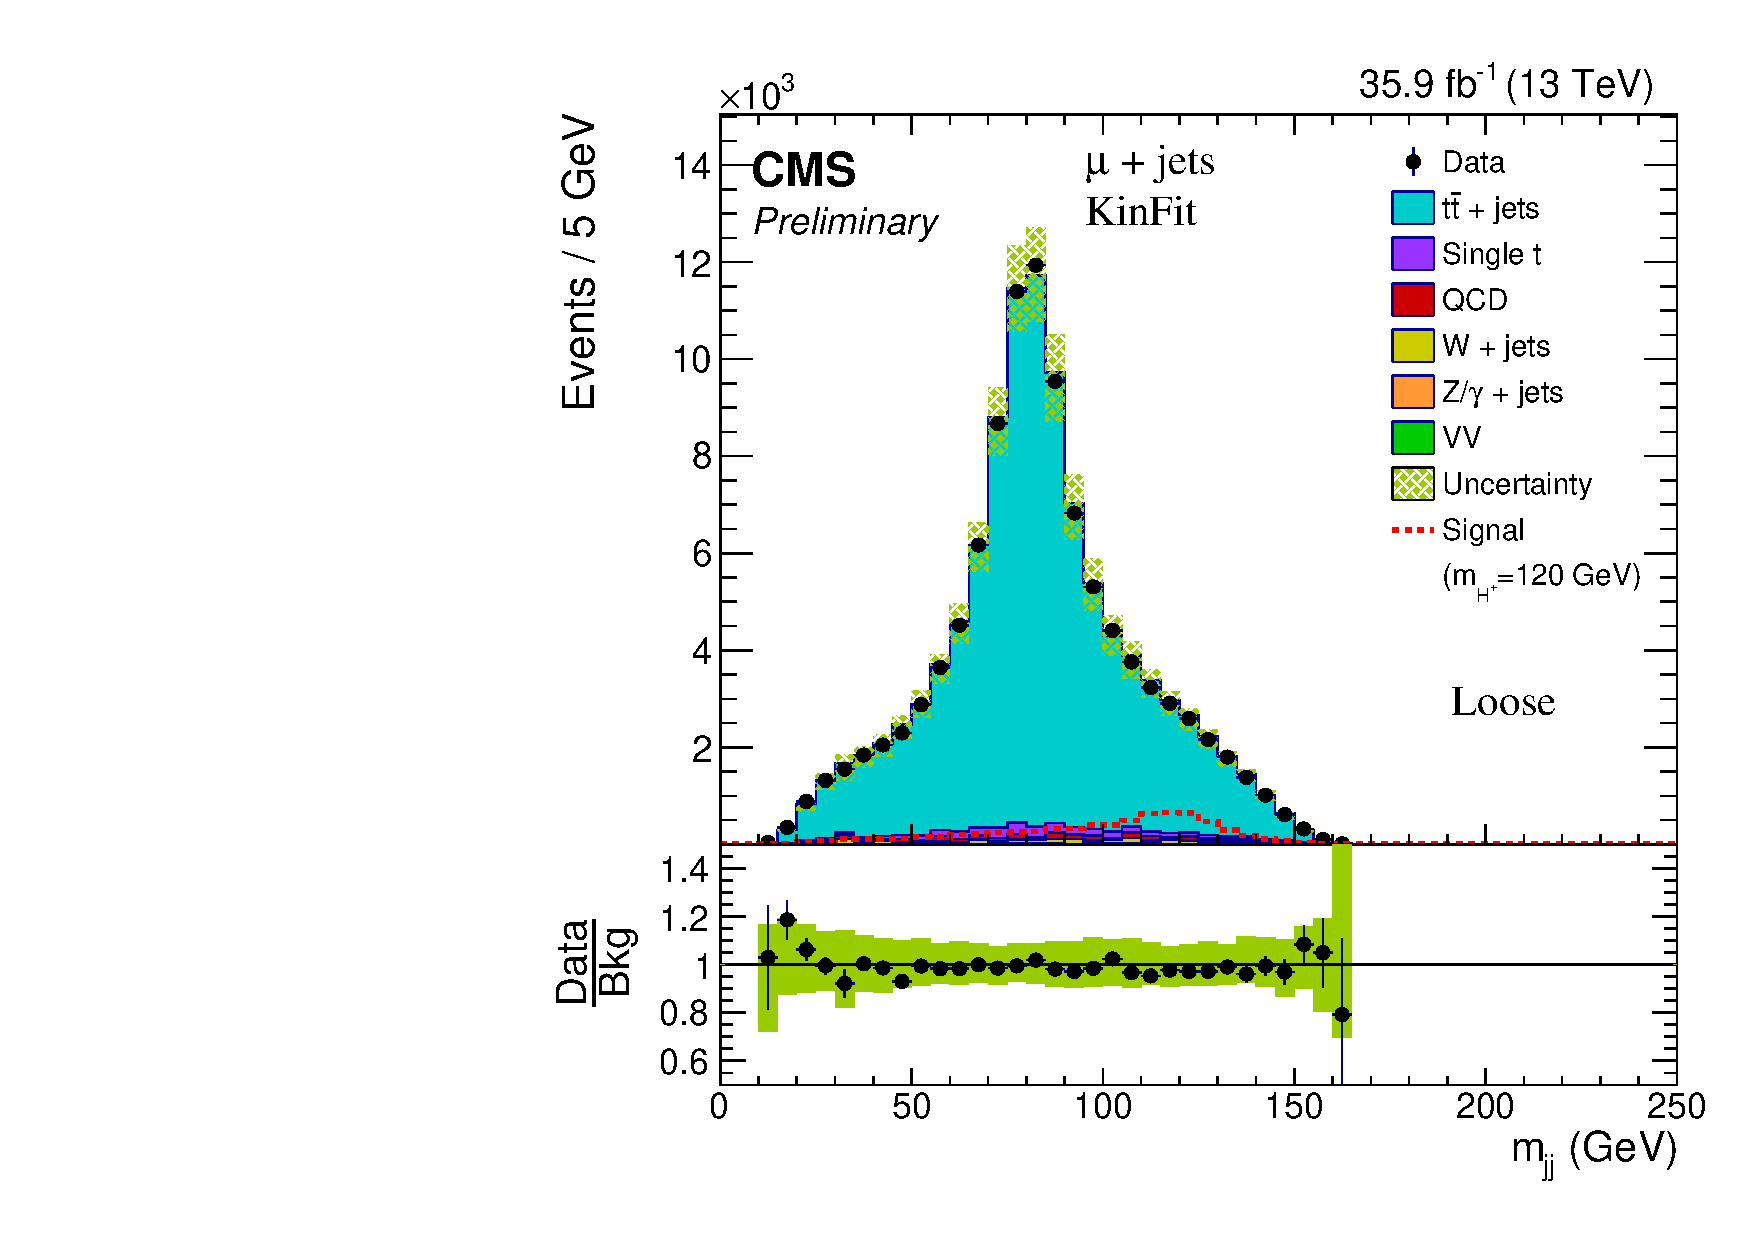
\includegraphics[width=0.40\linewidth]{Image/Muon/KinFit/mjj_kfit_CTagExL_muKinFit.pdf}}
\subfigure[]
{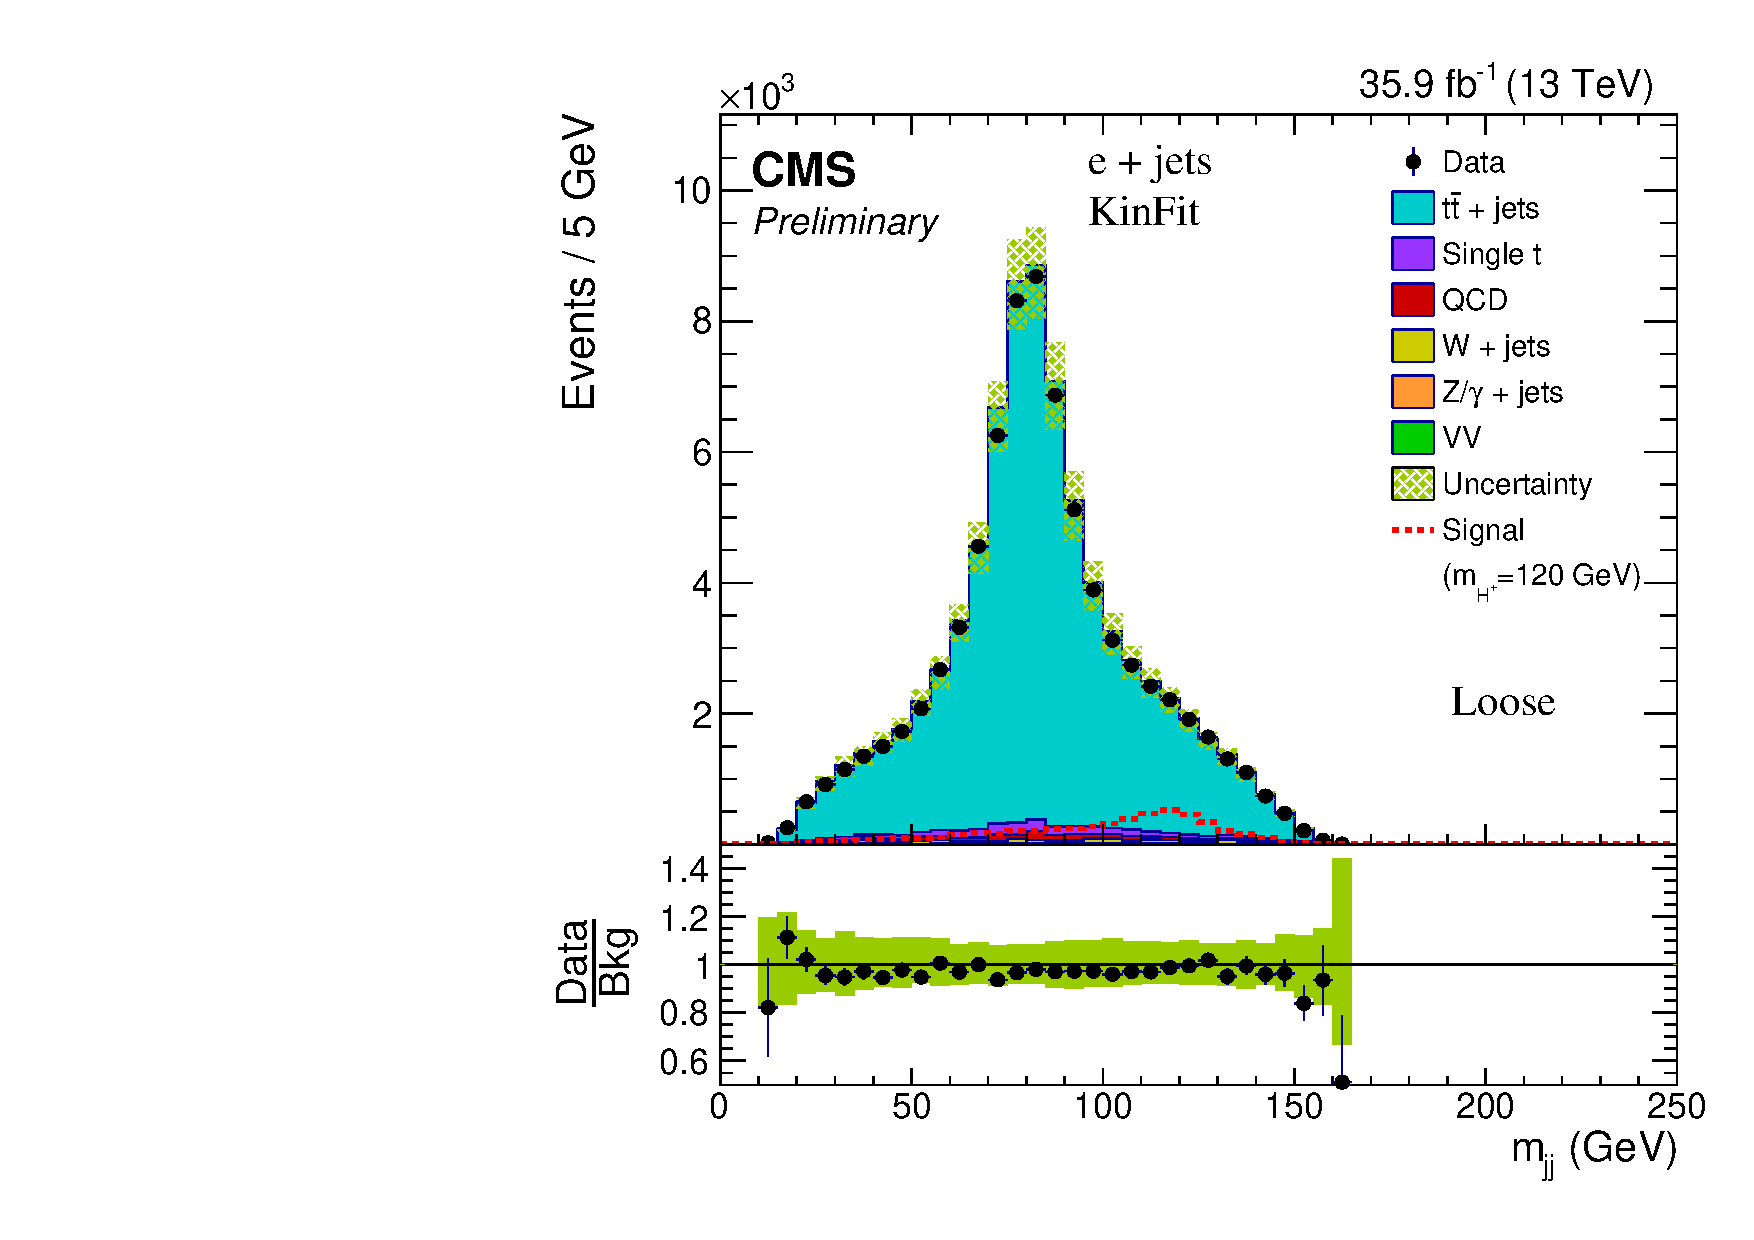
\includegraphics[width=0.40\linewidth]{Image/Electron/KinFit/mjj_kfit_CTagExL_eleKinFit.pdf}}
\vfil
\subfigure[]
{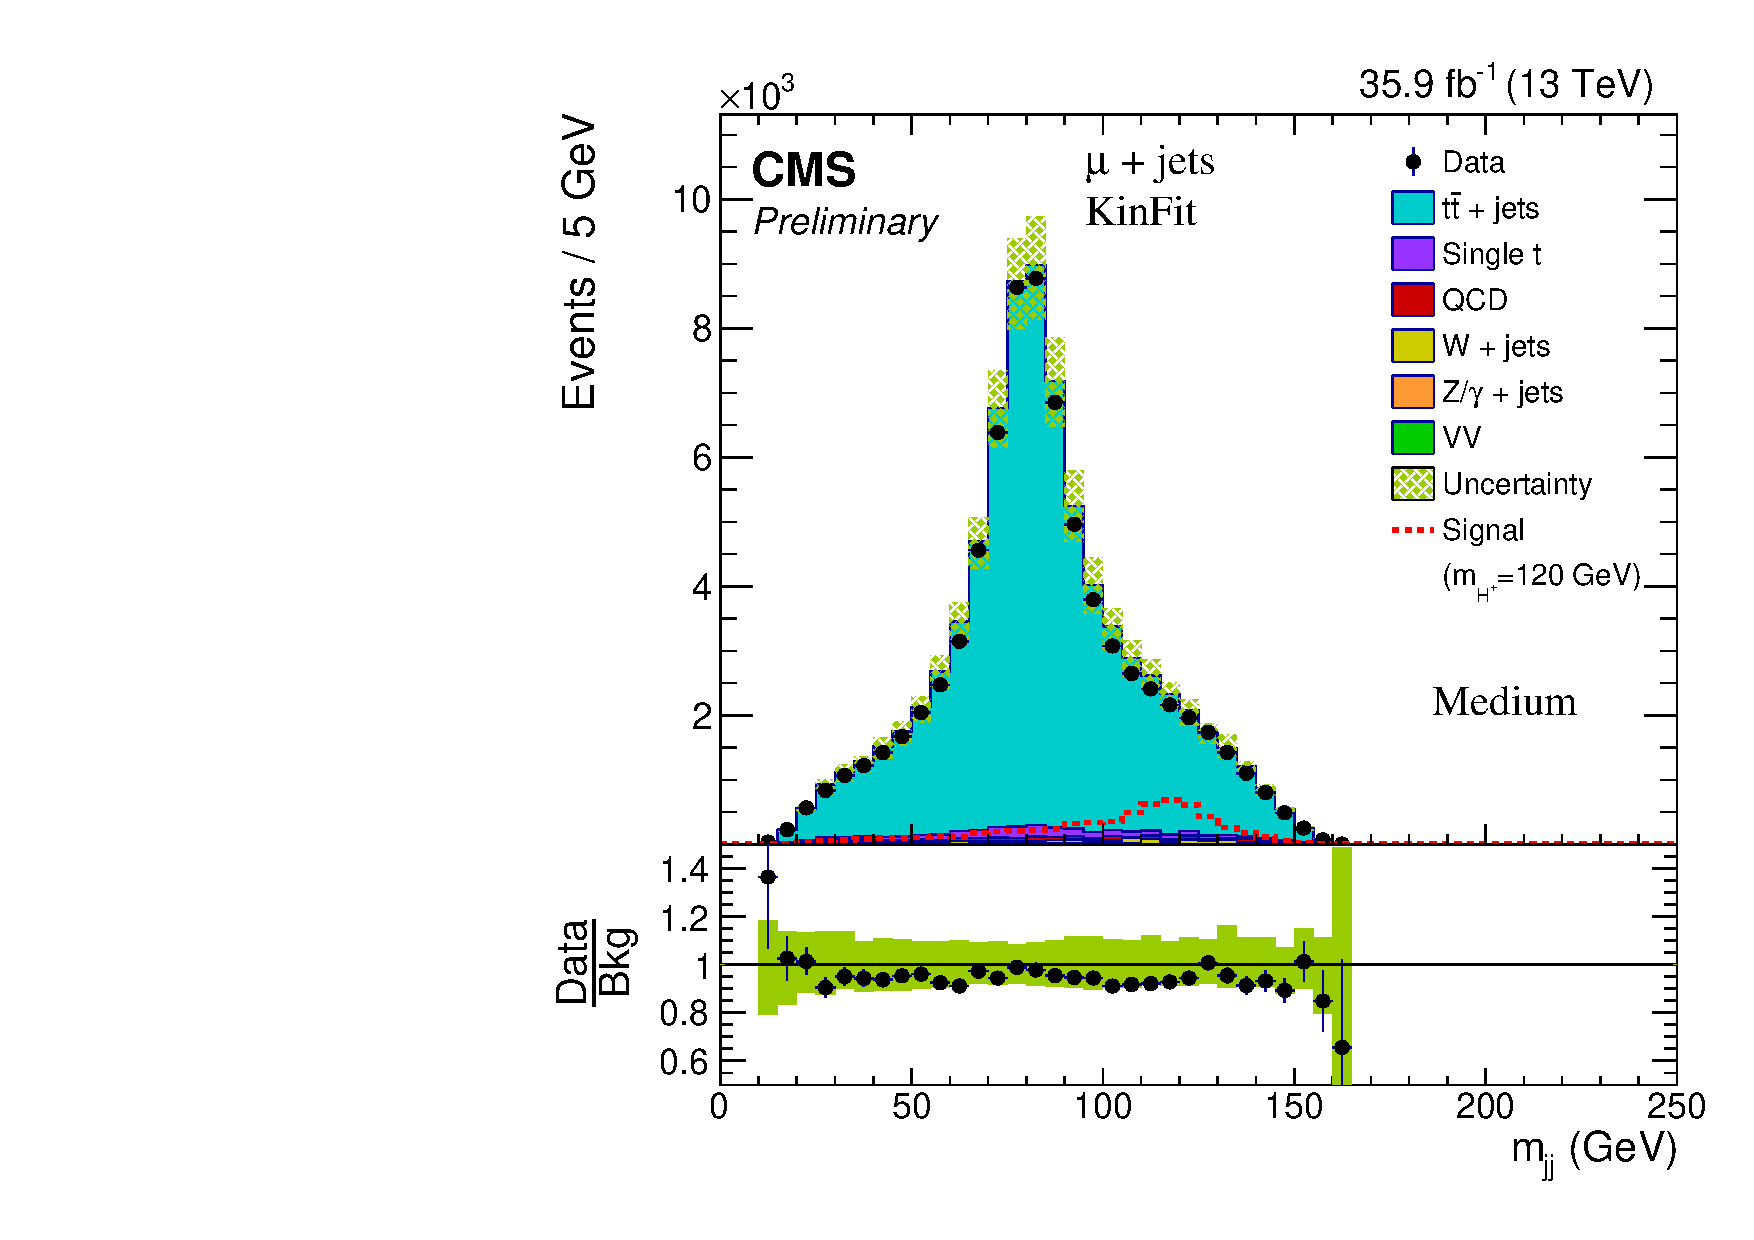
\includegraphics[width=0.40\linewidth]{Image/Muon/KinFit/mjj_kfit_CTagExM_muKinFit.pdf}}
\subfigure[]
{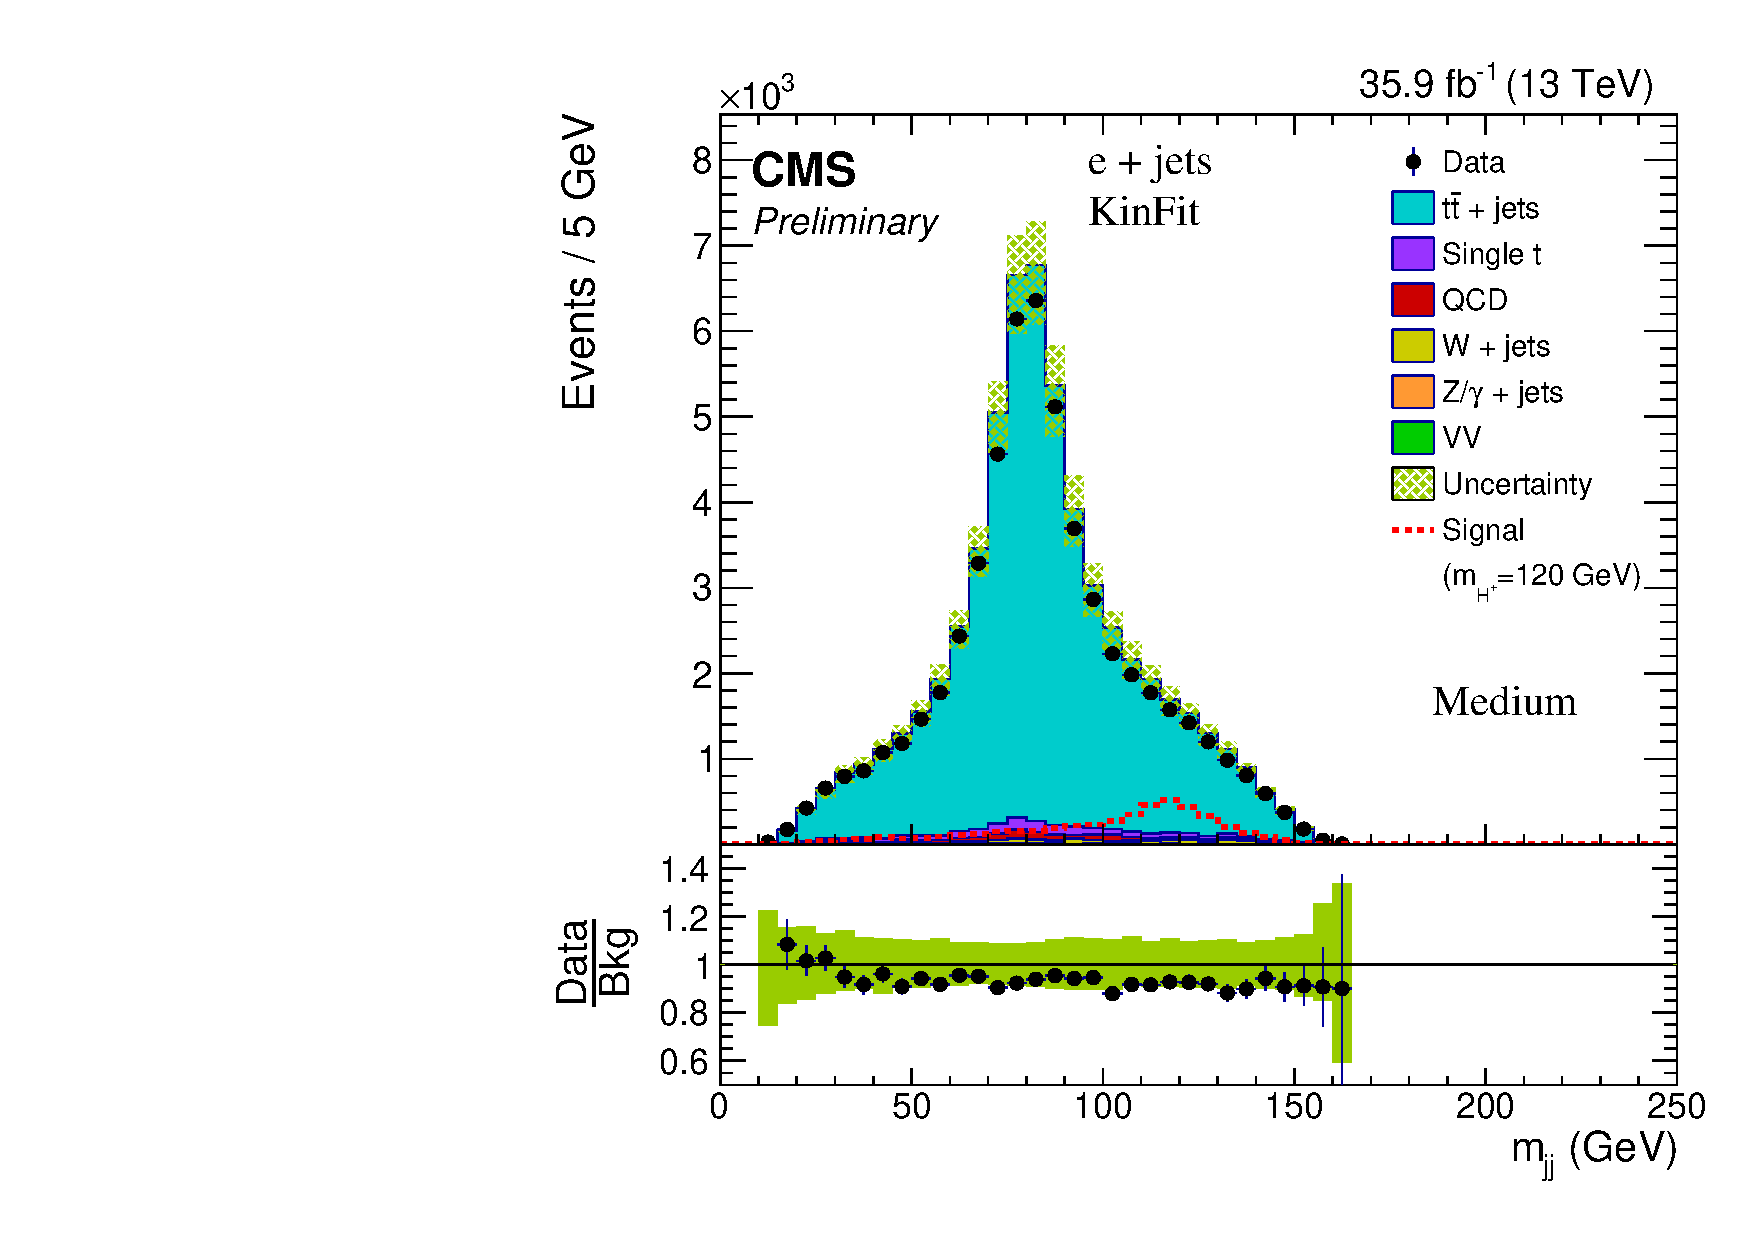
\includegraphics[width=0.40\linewidth]{Image/Electron/KinFit/mjj_kfit_CTagExM_eleKinFit.pdf}}
\vfil
\subfigure[]
{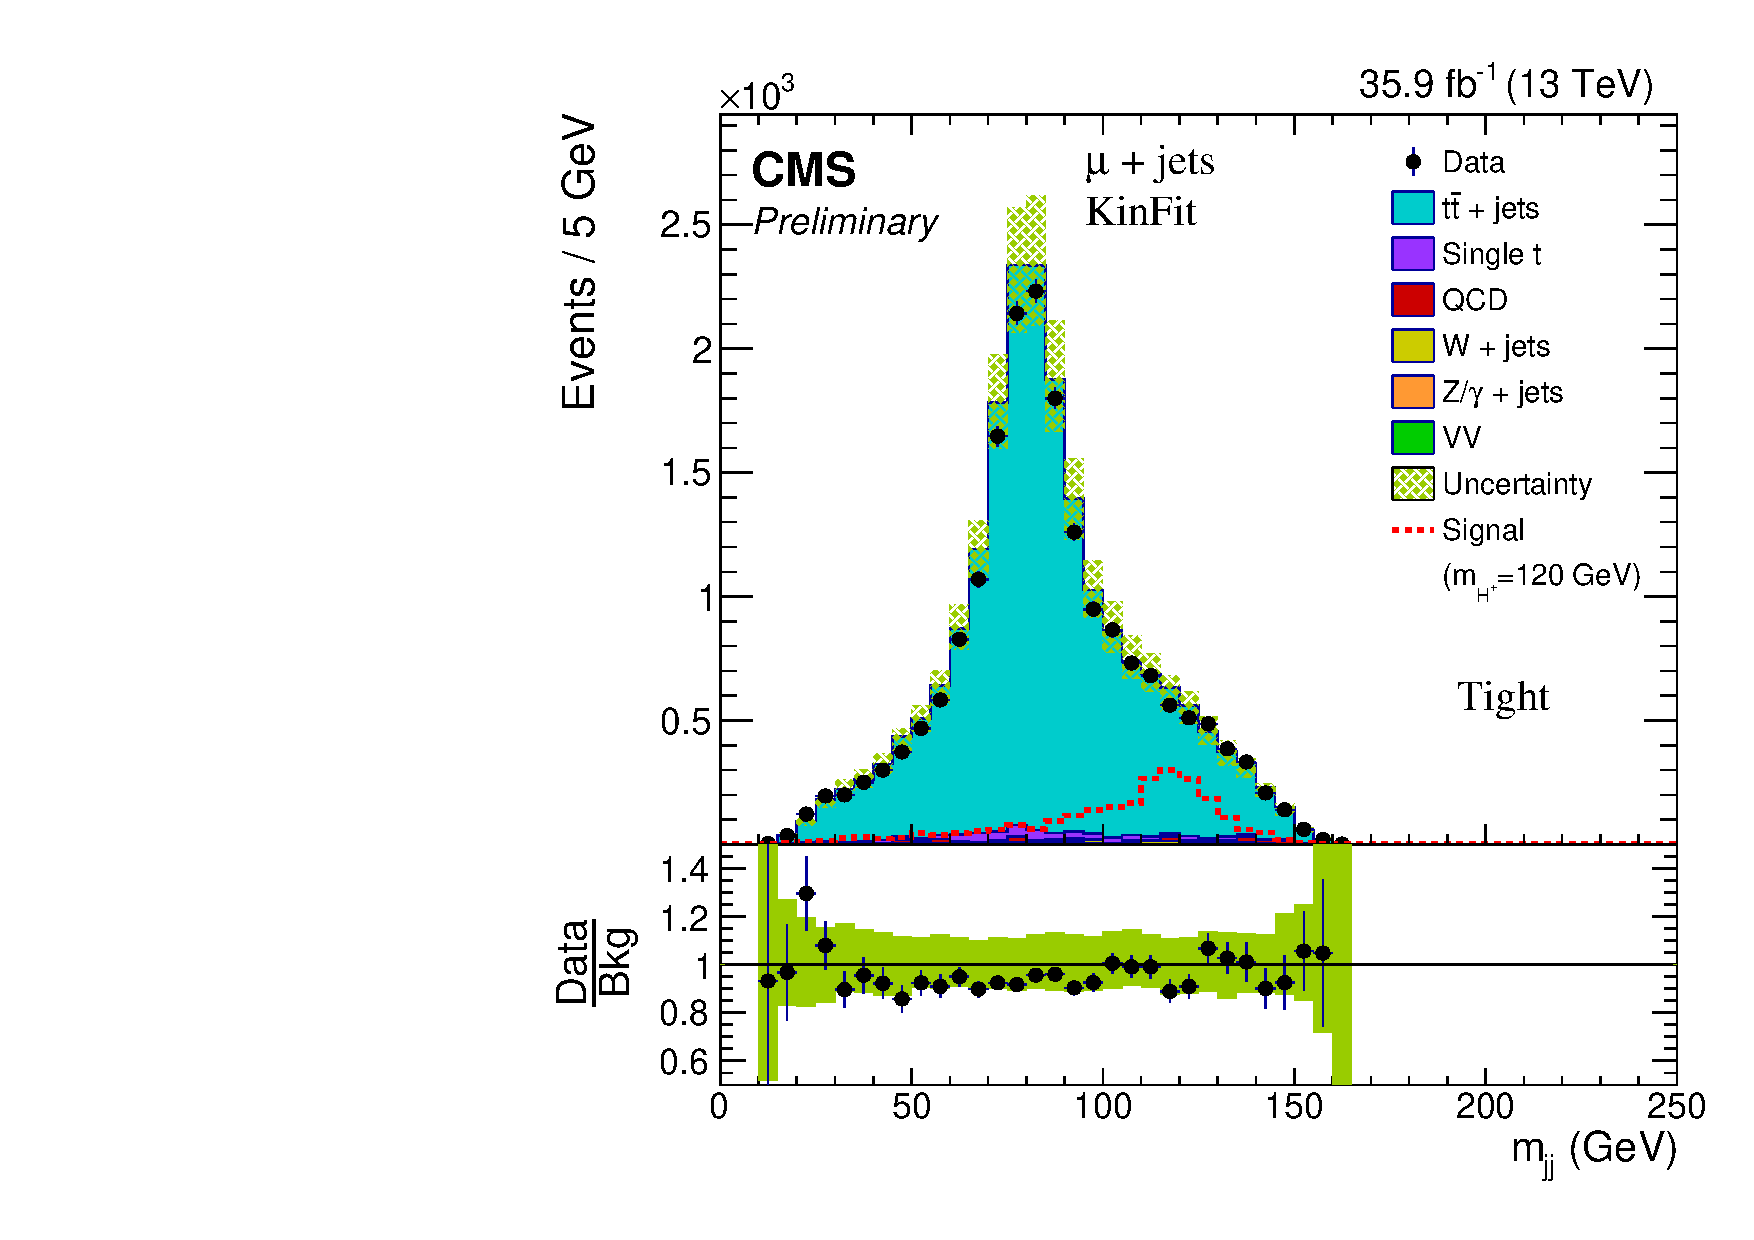
\includegraphics[width=0.40\linewidth]{Image/Muon/KinFit/mjj_kfit_CTagExT_muKinFit.pdf}}
\subfigure[]
{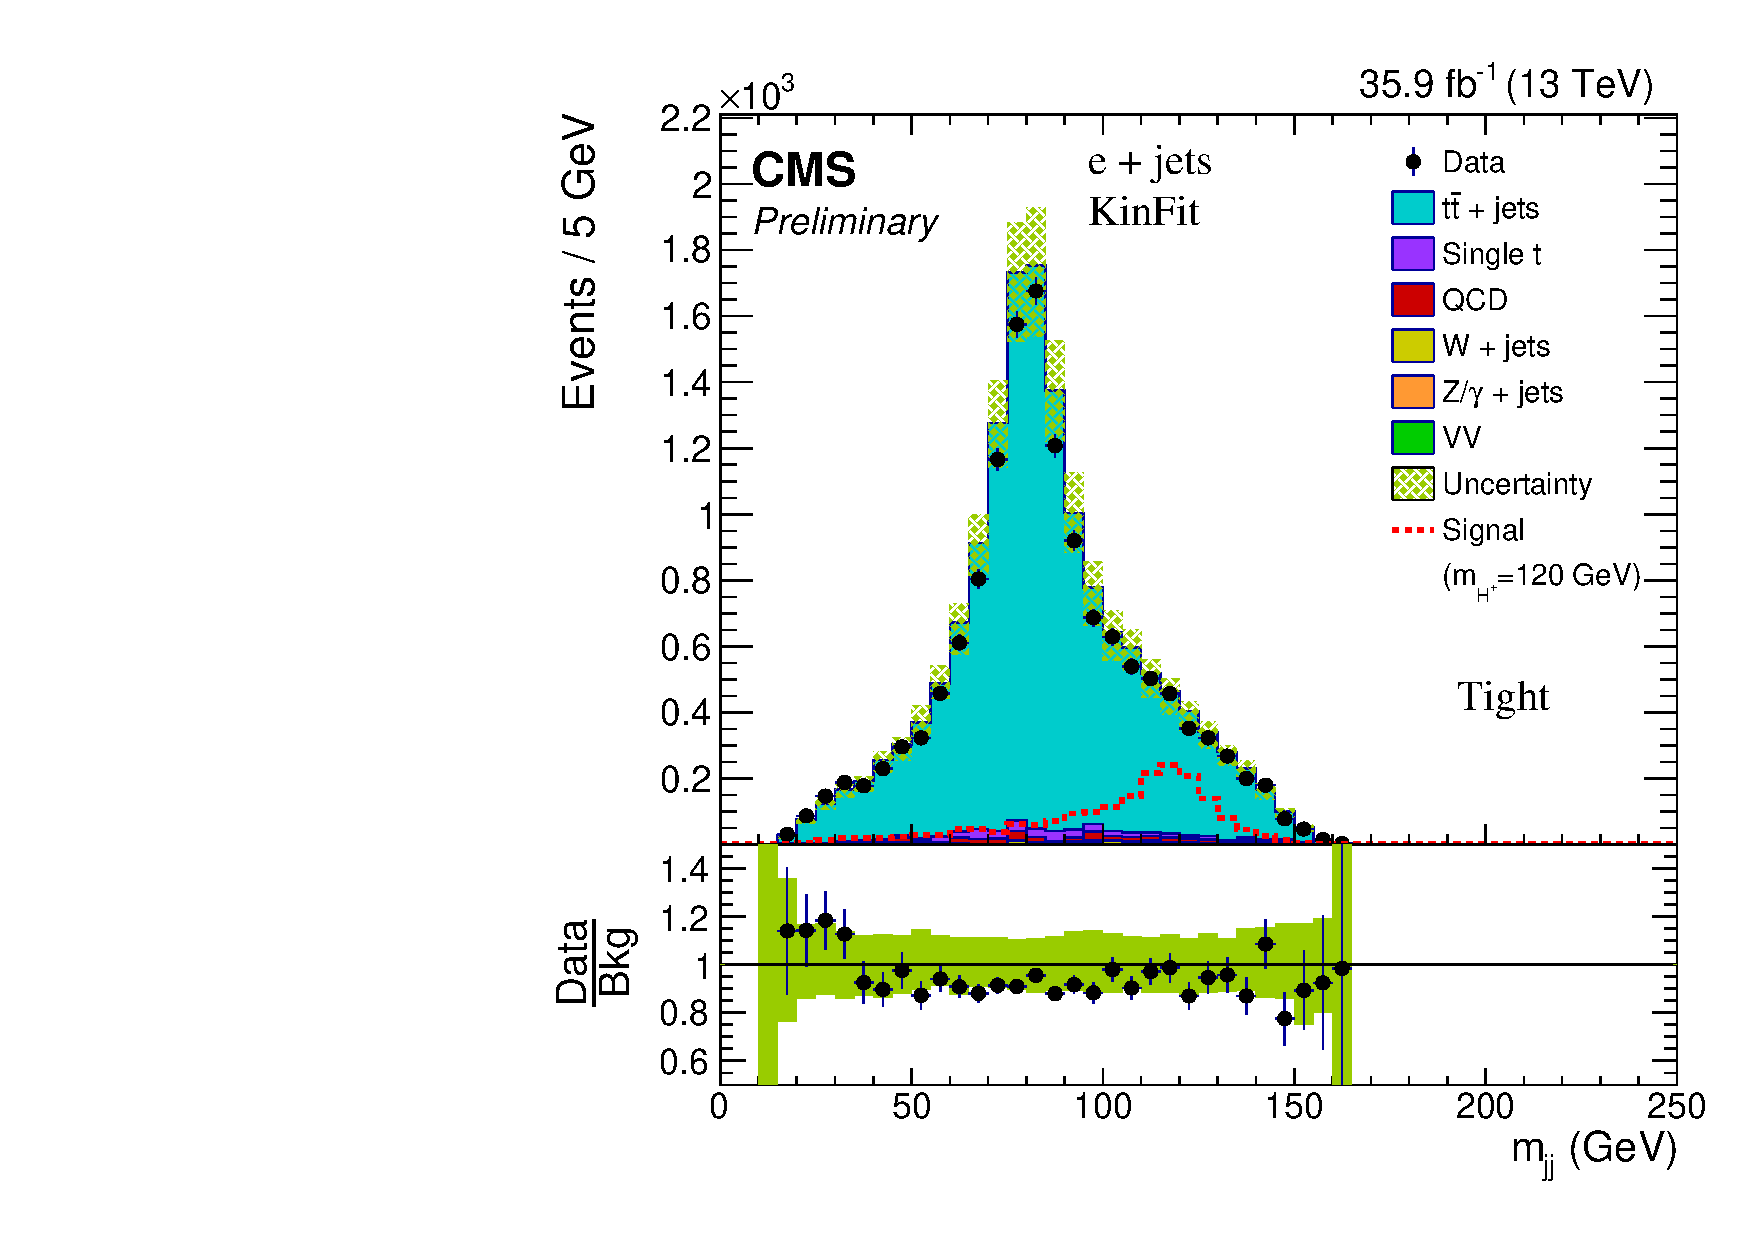
\includegraphics[width=0.40\linewidth]{Image/Electron/KinFit/mjj_kfit_CTagExT_eleKinFit.pdf}}
\caption{Distribution of $\mjj$ from exclusive charm categories as described in
Section~\ref{ss:mjj_cTagEx} for \mujets and \ejets channel. The signal significance is different across different
exclusive categories.}
\label{fig:mjj_cTagEx}
\end{figure}
\begin{table}
\caption{Event yield from exclusive charm categories after kinematic fit selection. The 
statistical uncertainty in the total background corresponds to the quadratically added 
uncertainties from individual backgrounds. However, a systematic uncertainty correlated 
among each background is linearly added for the total background. And each uncorrelated 
systematic uncertainty for the total background is quadratically added.}
\label{tab:eventYieldCTagEx}
\centering
\begin{adjustbox}{max width=\textwidth}
\begin{tabular}{cccccccc}
\hline 
\hline 
\multicolumn{1}{c}{{\bf{Process}}} & \multicolumn{2}{c}{{Exclusive loose category}} & \multicolumn{2}{c}{{Exclusive medium category}} & \multicolumn{2}{c}{{Exclusive tight category}} \\
& $N_{\rm{events}}\pm \rm{stat}\pm \rm{sys}$ & $N_{\rm{events}} \pm \rm{stat} \pm \rm{sys}$ & $N_{\rm{events}} \pm \rm{stat} \pm \rm{sys}$ & $N_{\rm{events}} \pm \rm{stat} \pm \rm{sys}$ & $N_{\rm{events}} \pm \rm{stat} \pm \rm{sys}$ & $N_{\rm{events}} \pm \rm{stat} \pm \rm{sys}$\\
 & \mujets &  \ejets & \mujets &  \ejets & \mujets &  \ejets \\
\hline 
\hline 
$\mHp=80$ \GeV & 7171 $\pm$ 75 $\pm$ 678 & 5375 $\pm$ 64 $\pm$ 499 & 6137 $\pm$ 71 $\pm$ 551 & 4683 $\pm$ 61 $\pm$ 435 & 2471 $\pm$ 43 $\pm$ 278 & 1826 $\pm$ 37 $\pm$ 203\\
$\mHp=90$ \GeV & 7171 $\pm$ 74 $\pm$ 718 & 5556 $\pm$ 64 $\pm$ 535 & 6300 $\pm$ 72 $\pm$ 602 & 4818 $\pm$ 62 $\pm$ 468 & 2442 $\pm$ 42 $\pm$ 274 & 1843 $\pm$ 37 $\pm$ 208\\
$\mHp=100$ \GeV & 7382 $\pm$ 75 $\pm$ 718 & 5480 $\pm$ 64 $\pm$ 519 & 6591 $\pm$ 73 $\pm$ 638 & 4911 $\pm$ 62 $\pm$ 413 & 2570 $\pm$ 43 $\pm$ 290 & 1967 $\pm$ 38 $\pm$ 218\\
$\mHp=120$ \GeV & 7073 $\pm$ 73 $\pm$ 689 & 5291 $\pm$ 63 $\pm$ 524 & 6378 $\pm$ 72 $\pm$ 602 & 4732 $\pm$ 61 $\pm$ 410 & 2466 $\pm$ 42 $\pm$ 261 & 1923 $\pm$ 37 $\pm$ 213\\
$\mHp=140$ \GeV & 5716 $\pm$ 66 $\pm$ 625 & 4338 $\pm$ 57 $\pm$ 439 & 5043 $\pm$ 64 $\pm$ 507 & 3816 $\pm$ 55 $\pm$ 401 & 1869 $\pm$ 37 $\pm$ 208 & 1472 $\pm$ 32 $\pm$ 167\\
$\mHp=150$ \GeV & 4218 $\pm$ 57 $\pm$ 477 & 3215 $\pm$ 49 $\pm$ 363 & 3584 $\pm$ 54 $\pm$ 403 & 2774 $\pm$ 47 $\pm$ 317 & 1233 $\pm$ 30 $\pm$ 154 & 1015 $\pm$ 27 $\pm$ 135\\
$\mHp=155$ \GeV & 3447 $\pm$ 52 $\pm$ 416 & 2522 $\pm$ 44 $\pm$ 333 & 2758 $\pm$ 48 $\pm$ 357 & 2205 $\pm$ 43 $\pm$ 293 & 935 $\pm$ 27 $\pm$ 150 & 762 $\pm$ 24 $\pm$ 98\\
$\mHp=160$ \GeV & 2593 $\pm$ 45 $\pm$ 315 & 2053 $\pm$ 39 $\pm$ 249 & 2210 $\pm$ 43 $\pm$ 296 & 1699 $\pm$ 37 $\pm$ 244 & 682 $\pm$ 22 $\pm$ 105 & 506 $\pm$ 19 $\pm$ 65\\
\hline 
SM \ttjets & 100295 $\pm$ 195 $\pm$ 9239 & 74479 $\pm$ 166 $\pm$ 6851 & 76226 $\pm$ 178 $\pm$ 7396 & 56556 $\pm$ 152 $\pm$ 5472 & 19728 $\pm$ 86 $\pm$ 2319 & 14528 $\pm$ 73 $\pm$ 1641\\
Single \PQt & 2861 $\pm$ 29 $\pm$ 326 & 2159 $\pm$ 25 $\pm$ 261 & 2126 $\pm$ 27 $\pm$ 248 & 1585 $\pm$ 23 $\pm$ 189 & 483 $\pm$ 13 $\pm$ 65 & 355 $\pm$ 11 $\pm$ 48\\
QCD multijet & 1772 $\pm$ 140  & 1402 $\pm$ 108 & 1067 $\pm$ 124 & 1077 $\pm$ 109 & 202 $\pm$ 56 & 296 $\pm$ 54 \\
\wjets & 1609 $\pm$ 109 $\pm$ 369 & 1181 $\pm$ 54 $\pm$ 191 & 1131 $\pm$ 57 $\pm$ 282 & 792 $\pm$ 46 $\pm$ 136 & 144 $\pm$ 19 $\pm$ 43 & 110 $\pm$ 16 $\pm$ 34\\
\dyjets & 198 $\pm$ 12 $\pm$ 45 & 250 $\pm$ 11 $\pm$ 52 & 143 $\pm$ 9 $\pm$ 35 & 153 $\pm$ 9 $\pm$ 33 & 61 $\pm$ 6 $\pm$ 14 & 35 $\pm$ 5 $\pm$ 7\\
VV & 70 $\pm$ 15 $\pm$ 10 & 52 $\pm$ 11 $\pm$ 12 & 68 $\pm$ 14 $\pm$ 27 & 16 $\pm$ 6 $\pm$ 9 & 14 $\pm$ 6 $\pm$ 7 & 4 $\pm$ 4 $\pm$ 1\\
\hline 
All background & 106805 $\pm$ 266 $\pm$ 9932 & 79523 $\pm$ 207 $\pm$     7346 & 80761 $\pm$ 226 $\pm$ 7915 & 60179 $\pm$ 194 $\pm$ 5826 & 20632   $\pm$ 106 $\pm$ 2420 & 15329 $\pm$ 93 $\pm$ 1718\\
\hline 
Data & 105485 $\pm$ 325 & 77244 $\pm$ 278 & 76811 $\pm$ 277 & 56051 $\pm$ 237 & 19451 $\pm$ 139 & 14179 $\pm$ 119 \\
\hline 
\end{tabular}
\end{adjustbox}
\end{table}

